\documentclass[
	% -- opções da classe memoir --
	12pt,				% tamanho da fonte
	openright,			% capítulos começam em pág ímpar (insere página vazia caso preciso)
	twoside,			% para impressão em verso e anverso. Oposto a oneside
	a4paper,			% tamanho do papel. 
	% -- opções da classe abntex2 --
	chapter=TITLE,		% títulos de capítulos convertidos em letras maiúsculas
	section=TITLE,		% títulos de seções convertidos em letras maiúsculas
	%subsection=TITLE,	% títulos de subseções convertidos em letras maiúsculas
	%subsubsection=TITLE,% títulos de subsubseções convertidos em letras maiúsculas
	% -- opções do pacote babel --
	english,			% idioma adicional para hifenização
	brazil				% o último idioma é o principal do documento
	]{abntex2}

% ---
% Pacotes básicos 
% ---
\usepackage{uarial}				% Usa a fonte Latin Modern			lmodern
\usepackage[T1]{fontenc}		% Selecao de codigos de fonte.
\usepackage[utf8]{inputenc}		% Codificacao do documento (conversão automática dos acentos)
\usepackage{lastpage}			% Usado pela Ficha catalográfica
\usepackage{indentfirst}		% Indenta o primeiro parágrafo de cada seção.
\usepackage{color}				% Controle das cores
\usepackage{graphicx}			% Inclusão de gráficos
\usepackage{microtype} 			% para melhorias de justificação

% pacotes adicionados
\usepackage{amsmath}
\usepackage{amssymb,amsfonts,amsthm}
\usepackage{setspace}
\usepackage{booktabs}
\usepackage[hyphens]{url}
% ---
		
% ---
% Pacotes adicionais, usados apenas no âmbito do Modelo Canônico do abnteX2
% ---
\usepackage{lipsum}				% para geração de dummy text
% ---
\usepackage{todonotes}
% ---
% Pacotes de citações
% ---
\usepackage[brazilian,hyperpageref]{backref}	 % Paginas com as citações na bibl
\usepackage[alf]{abntex2cite}	% Citações padrão ABNT


\renewcommand{\bf}[1]{\mathbf{#1}}
\renewcommand{\rm}[1]{\mathrm{#1}}

\usepackage{cite}
\renewcommand\citeleft{[}
\renewcommand\citeright{]}

\usepackage{listings}
\usepackage{color}
\definecolor{lightgray}{rgb}{.9,.9,.9}
\definecolor{darkgray}{rgb}{.4,.4,.4}
\definecolor{purple}{rgb}{0.65, 0.12, 0.82}

\lstdefinelanguage{JavaScript}{
  keywords={typeof, new, true, false, catch, function, return, null, catch, switch, var, if, in, while, do, else, case, break},
  keywordstyle=\color{blue}\bfseries,
  ndkeywords={class, export, boolean, throw, implements, import, this},
  ndkeywordstyle=\color{darkgray}\bfseries,
  identifierstyle=\color{black},
  sensitive=false,
  comment=[l]{//},
  morecomment=[s]{/*}{*/},
  commentstyle=\color{purple}\ttfamily,
  stringstyle=\color{red}\ttfamily,
  morestring=[b]',
  morestring=[b]"
}

\lstset{
   language=JavaScript,
   backgroundcolor=\color{lightgray},
   extendedchars=true,
   basicstyle=\footnotesize, 
   frame=tb,
   showstringspaces=false,
   showspaces=false,
   numbers=left,
   numberstyle=\footnotesize,
   numbersep=9pt,
   tabsize=2,
   breaklines=true,
   showtabs=false,
   captionpos=b,
   xleftmargin=.15\textwidth, 
   xrightmargin=.15\textwidth,
   aboveskip=3em,
   belowcaptionskip=3em
}

% --- 
% MUDAR CAPA E FOLHA DE ROSTO
% --- 

% \renewcommand{\imprimircapa}{
% \include{modelos/capa}}

% \renewcommand{\imprimirfolhaderosto}{
% 
\begin{center}

    {\large LUCAS RINALDI\\}
    \vspace{8cm}
    {\Large \textsc\textbf{{SISTEMA DE ATENDIMENTO AO CONSUMIDOR UTILIZANDO A TECNOLOGIA WebRTC} }\\}
    \vspace{1cm}
    \hspace{.45\linewidth}
    \begin{minipage}{.50\linewidth}

            \textbf{Trabalho apresentado ao Curso de Sistemas de Informação da Universidade Federal de Santa Catarina como requisito parcial para obtenção do grau de Bacharel em Sistemas de Informação.}

           
    
    \end{minipage}

    \vspace{2cm}
    \vfill
    {\large Florianópolis, Maio de 2016}
\end{center}

}

% --- 
% CONFIGURAÇÕES DE PACOTES
% --- 

% ---
% Configurações do pacote backref
% Usado sem a opção hyperpageref de backref
\renewcommand{\backrefpagesname}{Citado na(s) página(s):~}
% Texto padrão antes do número das páginas
\renewcommand{\backref}{}
% Define os textos da citação
\renewcommand*{\backrefalt}[4]{
	\ifcase #1 %
		Nenhuma citação no texto.%
	\or
		Citado na página #2.%
	\else
		Citado #1 vezes nas páginas #2.%
	\fi}%
% ---

% ---
% Configurações de aparência do PDF final

% alterando o aspecto da cor azul
\definecolor{blue}{RGB}{41,5,195}

% informações do PDF
\makeatletter
\hypersetup{
     	%pagebackref=true,
		colorlinks=true,       		% false: boxed links; true: colored links
    	linkcolor=blue,          	% color of internal links
    	citecolor=black,        		% color of links to bibliography
    	filecolor=magenta,      		% color of file links
		urlcolor=blue,
		bookmarksdepth=4
}

\makeatother
% --- 

% --- 
% Espaçamentos entre linhas e parágrafos 
% --- 

% O tamanho do parágrafo é dado por:
\setlength{\parindent}{1.3cm}

% Controle do espaçamento entre um parágrafo e outro:
\setlength{\parskip}{0.2cm}  % tente também \onelineskip

% ---
% Informações de dados para CAPA e FOLHA DE ROSTO
% ---
%Framework para a execução concorrente e multicomputada de algoritmos genéticos
\titulo{Sistema de Atendimento ao Consumidor Utilizando a Tecnologia WebRTC}
\autor{Lucas Rinaldi}
\local{Florianópolis}
\data{2018}
\orientador{Prof. Frank Siqueira}
%\coorientador{Equipe \abnTeX}
\instituicao{%
  Universidade Federal de Santa Catarina -- UFSC
  \par
  Centro Tecnológico -- CTC
  \par
  Departamento de Informática e Estatística -- INE}
\tipotrabalho{Trabalho de Graduação}
% O preambulo deve conter o tipo do trabalho, o objetivo, 
% o nome da instituição e a área de concentração 
\preambulo{Trabalho apresentado ao Curso de Sistemas de Informação da Universidade Federal de Santa Catarina como requisito parcial para obtenção do grau de Bacharel em Sistemas de Informação.}
%\preambulo{Projeto apresentado como requisito parcial para a obtenção do grau de Bacharel em Sistemas de Informação.}
% ---

% ---
% compila o indice
% ---
\makeindex
% ---

% ----
% Início do documento
% ----
\begin{document}

% Seleciona o idioma do documento (conforme pacotes do babel)
%\selectlanguage{english}
\selectlanguage{brazil}

% Retira espaço extra obsoleto entre as frases.
\frenchspacing

% ----------------------------------------------------------
% ELEMENTOS PRÉ-TEXTUAIS
% ----------------------------------------------------------
\pretextual
% ----------------------------------------------------------
% ELEMENTOS PRÉ-TEXTUAIS
% ----------------------------------------------------------

% ---
% Capa
% ---
\imprimircapa
% ---

% ---
% Folha de rosto
% (o * indica que haverá a ficha bibliográfica)
% ---
\imprimirfolhaderosto
% ---

% % ---
% Inserir a ficha bibliografica
% ---

% Isto é um exemplo de Ficha Catalográfica, ou ``Dados internacionais de
% catalogação-na-publicação''. Você pode utilizar este modelo como referência. 
% Porém, provavelmente a biblioteca da sua universidade lhe fornecerá um PDF
% com a ficha catalográfica definitiva após a defesa do trabalho. Quando estiver
% com o documento, salve-o como PDF no diretório do seu projeto e substitua todo
% o conteúdo de implementação deste arquivo pelo comando abaixo:
%
% \begin{fichacatalografica}
%     \includepdf{fig_ficha_catalografica.pdf}
% \end{fichacatalografica}

\begin{fichacatalografica}
%	\sffamily
%	\vspace*{\fill}					% Posição vertical
%	\begin{center}					% Minipage Centralizado
%	\fbox{\begin{minipage}[c][8cm]{13.5cm}		% Largura
%	\small
%	\imprimirautor
%	%Sobrenome, Nome do autor
%	
%	\hspace{0.5cm} \imprimirtitulo  / \imprimirautor. --
%	\imprimirlocal, \imprimirdata-
%	
%	\hspace{0.5cm} \pageref{LastPage} p. : il. (algumas color.) ; 30 cm.\\
%	
%	\hspace{0.5cm} \imprimirorientadorRotulo~\imprimirorientador\\
%	
%	\hspace{0.5cm}
%	\parbox[t]{\textwidth}{\imprimirtipotrabalho~--~\imprimirinstituicao,
%	\imprimirdata.}\\
%	
%	\hspace{0.5cm}
%		1. Palavra-chave1.
%		2. Palavra-chave2.
%		2. Palavra-chave3.
%		I. Orientador.
%		II. Universidade xxx.
%		III. Faculdade de xxx.
%		IV. Título 			
%	\end{minipage}}
%	\end{center}
\end{fichacatalografica}
% ---
% RESUMOS
% ---

% resumo em português
\setlength{\absparsep}{18pt} % ajusta o espaçamento dos parágrafos do resumo
\begin{resumo}
O objetivo desse trabalho é melhorar a forma como e-commerce, suporte técnico e serviços online fornecem atendimento ao cliente implementando um sistema de comunicação por vídeo que possa ser incluído em websites de forma simples e rápida. Para a transmissão de vídeos em tempo real será utilizada a tecnologia WebRTC, que apesar de ser relativamente nova, está expandindo horizontes na questão de transmissão de vídeos. Essa tecnologia torna desnecessário o uso de plugins e bibliotecas externas para comunicação através de áudio e vídeo no browser, simplificando o acesso ao sistema de atendimento.

\textbf{Palavras-chaves}:  sistemas web, webrtc, redes ponto-a-ponto, vídeoconferência, suporte
\end{resumo}

% resumo em inglês
\begin{resumo}[Abstract]
 \begin{otherlanguage*}{english}
Resumo em Inglês
   \vspace{\onelineskip}
 
   \noindent 
   \textbf{Keywords}:Palavras Chaves.
 \end{otherlanguage*}
\end{resumo}

%% resumo em francês 
%\begin{resumo}[Résumé]
% \begin{otherlanguage*}{french}
%    Il s'agit d'un résumé en français.
% 
%   \textbf{Mots-clés}: latex. abntex. publication de textes.
% \end{otherlanguage*}
%\end{resumo}
%
%% resumo em espanhol
%\begin{resumo}[Resumen]
% \begin{otherlanguage*}{spanish}
%   Este es el resumen en español.
%  
%   \textbf{Palabras clave}: latex. abntex. publicación de textos.
% \end{otherlanguage*}
%\end{resumo}
% ---

% % ---
% Inserir errata
% ---
\begin{errata}
Elemento opcional da \citeonline[4.2.1.2]{NBR14724:2011}. Exemplo:

\vspace{\onelineskip}

FERRIGNO, C. R. A. \textbf{Tratamento de neoplasias ósseas apendiculares com
reimplantação de enxerto ósseo autólogo autoclavado associado ao plasma
rico em plaquetas}: estudo crítico na cirurgia de preservação de membro em
cães. 2011. 128 f. Tese (Livre-Docência) - Faculdade de Medicina Veterinária e
Zootecnia, Universidade de São Paulo, São Paulo, 2011.

\begin{table}[htb]
\center
\footnotesize
\begin{tabular}{|p{1.4cm}|p{1cm}|p{3cm}|p{3cm}|}
  \hline
   \textbf{Folha} & \textbf{Linha}  & \textbf{Onde se lê}  & \textbf{Leia-se}  \\
    \hline
    1 & 10 & auto-conclavo & autoconclavo\\
   \hline
\end{tabular}
\end{table}

\end{errata}
% ---

% % ---
% Inserir folha de aprovação
% ---

% Isto é um exemplo de Folha de aprovação, elemento obrigatório da NBR
% 14724/2011 (seção 4.2.1.3). Você pode utilizar este modelo até a aprovação
% do trabalho. Após isso, substitua todo o conteúdo deste arquivo por uma
% imagem da página assinada pela banca com o comando abaixo:
%
% \includepdf{folhadeaprovacao_final.pdf}
%
\begin{folhadeaprovacao}


\begin{center}


            {UNIVERSIDADE FEDERAL DE SANTA CATARINA} \\
           

    \vspace{1.5cm}
                                    {VICTOR COSTA MELO}\\
    \bfseries{}
\end{center}

Esta Monografia foi julgada adequada para a obten\c{c}\~{a}o do título  de Bacharel em Engenharia de Computação, sendo aprovada em sua forma final  pela banca examinadora:

    \vspace{2.5cm}
    \assinatura{Orientador(a): Prof. Dr. Analucia \\ Universidade Federal de Santa Catarina - UFSC}
    \assinatura{Prof. Dr. Huguinho \\ Universidade Federal de Santa Catarina - UFSC}
    \assinatura{Prof. Dr. Zezinho \\ Universidade Federal de Santa Catarina - UFSC}
    \assinatura{Prof. Dr. Luizinho \\ Universidade Federal de Santa Catarina - UFSC}
    \vspace{3 cm}%\vfill

    \begin{center}
        Araranguá, 12 de dezembro de 2016
    \end{center}
  
\end{folhadeaprovacao}
% % ---
% Dedicatória
% ---
\begin{dedicatoria}
   \vspace*{\fill}
   \centering
   \noindent
   \textit{ Este trabalho é dedicado às crianças adultas que,\\
   quando pequenas, sonharam em se tornar cientistas.} \vspace*{\fill}
\end{dedicatoria}
% ---
% % ---
% Agradecimentos
% ---
\begin{agradecimentos}
ou Acknowledgements, se em inglês \\
Opcional

\end{agradecimentos}
% ---
% % ---
% Epígrafe
% ---
\begin{epigrafe}
    \vspace*{\fill}
	\begin{flushright}
		\textit{``Não vos amoldeis às estruturas deste mundo, \\
		mas transformai-vos pela renovação da mente, \\
		a fim de distinguir qual é a vontade de Deus: \\
		o que é bom, o que Lhe é agradável, o que é perfeito.\\
		(Bíblia Sagrada, Romanos 12, 2)}
	\end{flushright}
\end{epigrafe}
% ---


% ---
% inserir o sumario
% ---
\pdfbookmark[0]{\contentsname}{toc}
\tableofcontents*
\cleardoublepage
% ---

% ---
% inserir lista de ilustrações
% ---
\pdfbookmark[0]{\listfigurename}{lof}
\listoffigures
\cleardoublepage
% ---

% ---
% inserir lista de tabelas
% ---
\pdfbookmark[0]{\listtablename}{lot}
\listoftables
\cleardoublepage
% ---

% ---
% inserir lista de abreviaturas e siglas
% ---
\pdfbookmark[0]{\listadesiglasname}{toc}
\begin{siglas}
  \addcontentsline{toc}{chapter}{\listadesiglasname}
  \item[AJAX] Asynchronous JavaScript and XML
  \item[API] Application Programming Interface
  \item[CGI] Common Gateway Interface
  \item[CSRF] Cross-site request forgery 
  \item[DOM] Document Object Model
  \item[HLS] HTTP Live Streaming
  \item[HTTP] Hypertext Transfer Protocol
  \item[HTTPS] Hypertext Transfer Protocol Secure
  \item[ICE] Interactive Connectivity Establishment
  \item[IETF] Internet Engineering Task Force
  \item[IP] Internet Protocol
  \item[NAT] Network Address Translator
  \item[PaaS] Platform as a Service
  \item[P2P] Peer-to-Peer
  \item[REST] Representational State Transfer
  \item[RF] Requisitos Funcionais
  \item[RNF] Requisitos Não-Funcionais
  \item[RPTM] Real-time Messaging Protocol
  \item[SAC] Serviço de Atendimento ao Consumidor
  \item[SOAP] Simple Object Access Protocol
  \item[SQL] Structured Query Language
  \item[SSL] Secure Sockets Layer
  \item[STUN] Session Traversal Utilities for NAT
  \item[TCP] Transmission Control Protocol
  \item[TI] Tecnologia da Informação
  \item[TLS] Transport Layer Security
  \item[TURN] Traversal Using Relays around NAT
  \item[UI] User Interface
  \item[URI] Uniform Resource Identifier
  \item[URL] Uniform Resource Locator
  \item[WSDL] Web Services Description Language
  \item[W3C] World Wide Web Consortium
\end{siglas}
\cleardoublepage
% ---

% ----------------------------------------------------------
% ELEMENTOS TEXTUAIS
% ----------------------------------------------------------
\textual

% ----------------------------------------------------------
% Introdução (obrigatório)
% ----------------------------------------------------------
\chapter[Introdução]{Introdução}\label{chap:introducao}

Com a crescente competitividade e concorrência de mercado, uma das maneiras de um negócio se destacar e conseguir sobreviver nesse realidade é investir no relacionamento com o cliente. Esse investimento busca melhorar o grau de satisfação do cliente, que possui um papel muito importante na longevidade do negócio.

Podemos identificar alguns problemas que afetam empresas no mercado atual em relação a este assunto:
\begin{itemize}
\item Empresas estão falhando em conhecer com precisão o perfil de seus consumidores; 
\item Há grande preocupação em adquirir novos clientes, mas não em retê-los. De acordo com \cite{marketingmetrics2015}, o preço para conseguir um novo cliente pode ser até 14 vezes maior que nutrir e manter um que já está na base;
\item A tecnologia no atendimento ao cliente resultou em impessoalidade, com cada vez mais robôs atendentes no lugar de pessoas.
\end{itemize}

Uma das maneiras utilizadas para realizar a comunicação com o cliente é através do Sistema de Atendimento ao Consumidor - mais conhecido como SAC - de cada empresa. O SAC pode ser visto como uma ferramenta para solucionar a grande demanda de dúvidas, solicitações e reclamações de sua base de clientes, consistindo em uma das possíveis estratégias para desenvolver um bom relacionamento com a base de clientes de uma empresa.

Dados trazidos por \cite{hbrdelightcustomer2010} mostram que 48\% dos consumidores que tiveram experiências negativas com o SAC contam a dez ou mais pessoas; enquanto somente 23\% com experiências positivas contam a dez ou mais pessoas. Passamos da fase em que o atendimento ao cliente é um mero suporte, e ser eficiente nesse processo pode garantir a longevidade do seu negócio.

Alguns problemas encontrados em sistemas de atendimento ao consumidor são:
\begin{itemize}
\item Um novo perfil de consumidor surgiu no mercado (os da Geração Y, ou Millennials). Esse perfil é mais fluído e versátil, exigindo inovação dos profissionais de atendimento \cite{salesforcestateofservice2015};
\item Burocracia gerada por processos e tecnologias engessadas e obsoletas criam fluxos confusos e exaustivos para os consumidores, deixando o SAC no passado e por consequência ineficiente;
\item As empresas não estão nos mesmos canais que os clientes e não conseguem acompanhar as mudanças rápidas que a Internet, as redes sociais e as novas tecnologias provocam nos consumidores todos os dias.
\item O principal meio de atendimento ainda é via telefone (de acordo com \cite{cenariodossacs2015}). O consumidor atual não se encaixa mais nesse perfil. Dados mostram que 58\% dos brasileiros não estão dispostos a esperar mais que 5 minutos por uma resposta ao telefone de um SAC.
\end{itemize}

Com base nas necessidades do mercado de um melhor relacionamento com o cliente, nas deficiências dos atuais sistemas de atendimento e nas limitações técnicas que alguns consumidores enfrentam, decidimos desenvolver um Sistema de Atendimento ao Consumidor que funcione através de transmissão de vídeo utilizando a tecnologia WebRTC.

\section{Motivação}
Observa-se a existência de diversas aplicações \textit{web} voltadas para atendimento ao consumidor, com foco em soluções de \textit{tickets}, análise e categorização dos mesmos. 

Entre elas é possível citar Zendesk\footnote{Disponível em: <https://www.zendesk.com/>. Acesso em 30 jun. 2017.} e Desk.com\footnote{Disponível em: <https://www.desk.com/>. Acesso em 30 jun. 2017.} como estado da arte desse segmento. O mesmo acontece no segmento de programas voltados para conversas através de vídeo. No estado da arte dessa categoria podemos citar appear.in\footnote{Disponível em: <https://www.appear.in/>. Acesso em 30 jun. 2017.}, disponível como aplicação web; Hangouts\footnote{Disponível em: <https://hangouts.google.com/>. Acesso em 30 jun. 2017.}, com versão Web e aplicativo móvel; e o Skype\footnote{Disponível em: <https://www.skype.com/>. Acesso em 30 jun. 2017.}, disponível para Web, \textit{desktop} e dispositivos móveis.

Entretanto a correlação dos dois segmentos é pouco explorado, tanto no âmbito da web, como com programas \textit{desktop}, ou seja, sem a necessidade de instalação de programas e \textit{plugins}.  Para o usuário, a facilidade de acesso e a independência do sistema operacional são vantagens de uma aplicação web em relação à sua versão para uma plataforma específica. 

Essa foi a principal motivação para este projeto: o desenvolvimento de uma aplicação web que faça a gerência de chamadas em vídeo e seja de fácil acesso para qualquer tipo de dispositivo. As chamadas iniciam-se por clientes que necessitam de assistência para o produto oferecido pela empresa, e são respondidas por atendentes designados para esse tipo de trabalho.

\section{Objetivo}
\subsection{Objetivo Geral}
Desenvolver um Sistema de Atendimento ao Consumidor que funcione através de transmissão de vídeo. O sistema deverá dispor de uma área administrativa, onde um profissional responsável por prestar atendimento gerenciará seus chamados.

\subsection{Objetivos Específicos}
Os seguintes objetivos específicos são almejados por este trabalho:
\begin{itemize}
	\item Estudar as soluções existentes para atendimento ao consumidor por chamadas de vídeo e identificar os problemas existentes;
	\item Desenvolver controle de acesso por parte dos atendentes.
	\item Desenvolver uma API baseada no modelo \textit{RESTful} para cadastro de usuários e chamadas através de um servidor HTTP.
	\item Desenvolver um módulo que oferece conexões através de \textit{WebSockets} para: 
    	\begin{itemize}
        	\item{Receber requisições de chamadas em vídeo \textit{realtime}.}
            \item{Realizar o \textit{handshake} necessário para conexão \textit{peer-to-peer} entre navegadores.}
      	\end{itemize}
	\item Implementar interface de aplicação web que suporte atualização em tempo real de componentes sem que seja necessário a atualização da página.
\end{itemize}

\section{Justificativa}
O programa desenvolvido será utilizado para resolver tanto problemas de negócio como problemas técnicos. Auxiliará no gerenciamento de chamadas de vídeo entre consumidores e profissionais de suporte/atendimento. Irá segurar chamadas, atendê-las e encerrá-las, mostrando dados e a localidade do cliente.

O modelo de atendimento por vídeo faz as empresas modernas retomarem a proximidade com os clientes. A tecnologia pode ser utilizada para sermos mais pessoais e alcançarmos uma gama maior de perfis de consumidor, por exemplo: o tipo de consumidor que está acostumado a interagir com o vídeo - meio de comunicação que se tornou uma das principais ferramentas de ajuda e comunicação na nossa sociedade atual. 

De acordo com \cite{customericare2015}, o vídeo é o canal de crescimento mais rápido. O número de chamadas de vídeo subiu de 600 milhões em 2010 para 30 bilhões em 2015. Enquanto isso, 2 bilhões de minutos de chamadas via Skype são feitos todos os dias e 36\% dos consumidores já expressam o desejo de terem suporte por meio de vídeo.

No entanto, a transmissão por vídeo é uma tecnologia relativamente nova em sistemas de atendimento, e somente 0,2\% das empresas prestam atendimento via vídeo (de acordo com a \cite{contactcentredoing2014}). 
Empresas de consultoria, da área da saúde, \textit{call} centers e advogados, por exemplo, já adotaram esse modelo. 

No âmbito jurídico, o vídeo já está sendo utilizado para colher depoimentos em processos. Para áreas de recursos humanos, diversas empresas utilizam a chamada por vídeo para realizar entrevistas com candidatos de outra localidade, sendo que aproximadamente 60\% do gerentes usam esse recurso (\cite{videochatinfographic2013}).

Já a transmissão de vídeo através de \textit{smartphones} e computadores pessoais não é um assunto tão recente. Utilizamos programas como Skype e \textit{plug-ins} de terceiros (ex.: Flash) para realizar chamadas entre dispositivos. Isso gera um \textit{overhead} para o consumidor, que fica a mercê da empresa para saber qual ferramenta utilizar para a chamada. Além disso, o usuário pode não ter em seu \textit{smartphone} o aplicativo ou \textit{plug-in} pré-instalado, e pode não dispor de espaço de armazenamento em seu dispositivo para realizar a instalação do software. O sistema desenvolvido precisará somente de um navegador (Google Chrome, Firefox, etc) em ambos nodos da conversação, ou seja, será suportado pela maioria dos \textit{smartphones}, computadores pessoais e \textit{tablets}. Assim, evitamos a necessidade de o usuário instalar programas adicionais em seu dispositivo.

\section{Metodologia}
Visando o sucesso deste projeto, foi adotada uma metodologia de trabalho que, no primeiro momento, consiste em reuniões periódicas com o orientador do trabalho de conclusão a fim de levantarmos requisitos e necessidades existentes do projeto.

Na segunda etapa foram realizadas análises de relatórios, artigos e pesquisas sobre dificuldades que consumidores têm em relação ao serviços de atendimento ao consumidor de uma grande parcela das empresas brasileiras. Foi observado que grande parte dos desejos e reclamações dos clientes dizem respeito à SACs com possibilidade de chamada em vídeo.

Com essa informação em mãos, uma pesquisa foi feita para encontrar as dificuldades que as empresas têm em fornecer um atendimento em vídeo de qualidade e fácil acesso. Análise feita em conjunto com sistemas utilizados para chamadas de videoconferência.

Para justificar a implementação do sistema foram levantados requisitos unindo as dificuldades tanto dos consumidores quanto das empresas em realizar chamados de assistência técnica bem sucedidos através da transmissão de vídeo. 

A solução encontrada diz respeito a um sistema que:
\begin{itemize}
\item Seja multi-dispositivo, ou seja, que funcione tanto em computadores pessoais como em dispositivos móveis;
\item Multi-plataforma, isto é, que esteja disponível em diversos sistemas operacionais, tanto para computadores (\textit{Windows}, \textit{Linux}, \textit{Mac OS}) quanto para dispositivos móveis (\textit{iOS}, \textit{Android});
\item Fácil ou nenhuma instalação, sem necessidade de instalação de aplicativos proprietários;
\item Possua gerenciamento de chamadas.
\end{itemize}

Construído o modelo e as ideias da aplicação, o projeto de implementação foi desenvolvido. O projeto constitui-se de análise de requisitos, descrição de tecnologias e arquitetura, junto das suas funcionalidades.

Com o projeto de implementação em mãos, o desenvolvimento do sistema será feito através de uma plataforma chamada \textit{NodeJS}, utilizando dois \textit{frameworks}: \textit{Express.js} e \textit{Socket.IO}, o primeiro responsável pela API e o segundo para conexão através de \textit{WebSockets}. O  servidor que fornece conexão por \textit{sockets} será responsável por realizar o estabelecimento da conexão entre dois nodos da rede, gerenciar chamadas e a API por guardar informações importantes sobre as mesmas.

Após a conexão entre duas partes a transmissão de mídia (principalmente vídeo) será realizada por uma tecnologia moderna chamada \textit{WebRTC}, especializada em transmissão de mídia em tempo real. 

Por fim, a publicação de todo sistema será feito através do \textit{Heroku}, uma empresa de \textit{PaaS} que fornece toda assistência para fornecer as aplicações online de forma simples e eficiente.

\section{Organização do Texto}
Conhecendo os objetivos, metodologia e a motivação por trás deste projeto, os próximos capítulos dão início às etapas de trabalho propostas.

Apresenta-se no capítulo seguinte a fundamentação teórica: descrições sobre os conceitos teóricos que cercam o sistema a ser implementado, descrição sobre conceitos utilizados por outras aplicações do mesmo ramo e a evolução da tecnologia que foi usada como base na construção do projeto (WebRTC); 

O terceiro capítulo contém uma análise das ferramentas existentes tanto na categoria de atendimento ao consumidor, como na de videoconferência, e uma breve discussão sobre os pontos de melhoria em comparação com este projeto.

No quarto capítulo é descrita a analise de requisitos do software, ou seja, as funcionalidades que serão implementadas no mesmo. Junto dos requisitos serão demonstradas a modelagem e a arquitetura do projeto.

A implementação do projeto encontra-se no quinto capítulo, no qual serão descritas a análise de requisitos, as decisões e descrições de tecnologias e ferramentas utilizadas, a arquitetura escolhida e as funcionalidades do sistema.

% ----------------------------------------------------------
% Fundamentação
% ----------------------------------------------------------
\chapter[Fundamentação Teórica]{Fundamentação Teórica}\label{chap:fundamentacao}

Para que seja possível uma completa compreensão do trabalho e de como usar o sistema por qualquer leitor, independentemente do nível de conhecimento sobre os principais tópicos do trabalho, é feita uma breve definição e elucidação destes tópicos nesse capítulo. Todos os conceitos descritos aqui assumem um prévio conhecimento do que é a Internet e a \textit{World Wide Web}.

\section{Arquitetura Cliente-Servidor}

Estilo de arquitetura criada para resolver o problema de distribuição de recursos. É uma estrutura onde existem dois tipos de participantes: o Cliente e Servidor, ambos denominados processos \cite{tanenbaum2002} dentro da arquitetura. 
 
Servidores são computadores (geralmente de alta performance) designados para atender requisições feitas através da Internet por clientes e também por outros servidores. Ao receber a requisição, o servidor é responsável por executar todo o trabalho solicitado ou retornar dados que o cliente necessita. É um componente que provê um serviço, uma função ou um recurso para o cliente.
 
Cliente e Servidor comunicam-se através de requisição e resposta. O Cliente emite uma requisição através de um protocolo de comunicação (por exemplo, protocolo HTTP) e o Servidor retorna uma resposta pelo mesmo caminho.
 
Existem diversos tipos de servidor, como por exemplo:
\begin{itemize}
	\item Servidor Web, responsável por servir arquivos estáticos ao cliente, carregando os mesmos de um disco rígido, geralmente através do protocolo HTTP.
    \item Servidor FTP, tem como responsabilidade transmitir arquivos ao cliente de maneira segura e sem corromper o arquivo.
    \item Servidor de E-mail, responsável por transmitir e guardar e-mails, utiliza o protocolo SMTP.
    \item Servidor Proxy, peça importante na distribuição de recursos, fica entre o Cliente e um outro Servidor (geralmente Web) e filtra requisições, melhora a performance e escolhe o melhor servidor para o cliente se conectar.
\end{itemize}
 
Essa arquitetura é uma peça importante pois elimina a necessidade do processamento de dados ser feito no computador do cliente \cite{clientserver1996}, possibilitando o uso e acesso de recursos por dispositivos de baixa performance.

\section{Arquitetura Peer-to-Peer}

Estilo de arquitetura que possui somente um tipo de entidade, essa definida de \textit{Servent} por \cite[Sec.~2]{p2pdefinition2001}. \textit{Servent} vem da junção das palavras \textit{Server} e \textit{Client}, indicando que cada \textit{peer} age como um cliente e um servidor. Dito isso, essa arquitetura permite que nodos heterogêneos e distintos possam comunicar-se entre si sem a necessidade de um servidor \cite{p2pgnutella2001}. 
 
Podemos ver pela Figura \ref{fig:clientserver_p2p} que a grande diferença dessa arquitetura para a cliente-servidor, é que a última possuí uma entidade de grande processamento, que possui todos os recursos e todos os nodos se conectam a ele, que é o Servidor.

\begin{figure}[ht!]
	\centering
		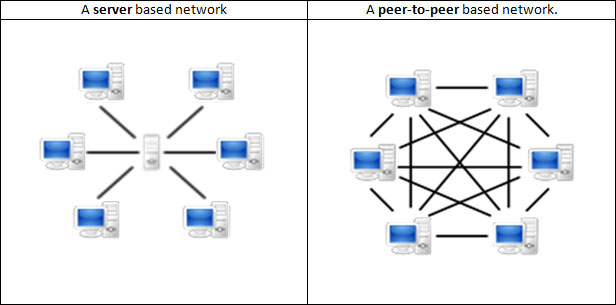
\includegraphics[scale=0.35]{figures/p2p-networks.jpg} 
	\caption{Arquiteturas de rede}
	\label{fig:clientserver_p2p}
\end{figure}

% Citando novamente \cite{p2pdefinition2001}, ele define dois tipos de arquitetura \textit{peer-to-peer}: a híbrida e a pura. A híbrida diz respeito à rede que possui uma entidade central (apesar de ser somente um nodo), a aplicação por trás da estrutura da rede dá a essa entidade mais "poderes" (estilo administrador). A pura como foi citada anteriormente é aquele que é formada somente por \textit{Servents}.
%FRANK: Essa categorização não me parece correta. Procure uma boa referência para isso. O parágrafo inteiro pode ser removido, se não for importante para o trabalho.
%LUCAS: A referencia esta nesse aqui {A definition of peer-to-peer networking}, mas acredito que não seja muito importante para o trabalho.

Podemos dizer então que uma arquitetura distribuída pode ser chamada de \textit{peer-to-peer} se cada um dos seus participantes compartilhar parte dos seus recursos, seja processamento,  armazenamento, banda larga. O que define quais recursos são, é o tipo de rede que está utilizando a arquitetura. 

\section{Arquitetura REST}

\textit{Representational State Transfer} (REST) é um estilo de arquitetura dedicado a sistemas distribuídos, que utiliza \textit{RESTful web services} (serviços Web compatíveis com REST) para facilitar a interoperabilidade de sistemas dentro de uma rede, como a Internet. O termo surgiu pela primeira vez no ano 2000 em uma dissertação de Roy Fielding, um dos principais autores da especificação HTTP.

De acordo com \cite{restroyfielding2000} a lógica por trás de uma arquitetura para \textit{Web} é descrita por um conjunto de restrições aplicadas aos elementos da arquitetura.

REST, utiliza padrões e restrições para definir como recursos da Internet devem ser definidos e utilizados. Algumas das restrições são:
\begin{itemize}
	\item Utilizar arquitetura cliente-servidor.
	\item Toda operação é \textit{stateless}, ou seja, não guarda estado; cada requisição ao servidor deve conter toda informação necessária para realizar a operação.
	\item O sistema deve implementar uma camada de \textit{cache} para melhorar a eficiência na rede (devido à natureza \textit{stateless}).
\end{itemize}

Interoperabilidade entre sistemas, significa acima de tudo a possibilidade de troca de informações dentro da arquitetura. Observamos na tabela \ref{table:elemento-de-dados-rest} a definição de elementos de dados que especificam o tipo de informação disponível e como chegar até ela.

\begin{table}[ht!]
	\centering
	\begin{tabular}{@{}ll@{}}
		\toprule
		\textbf{Elemento de dados}       & \textbf{Exemplos da web}       \\ \midrule
		\textit{resource}                & Mapeamento conceitual de uma referência em hipertexto   \\
		\textit{resource identifier}     & URL, URN, URI                                      \\
		\textit{representation}          & Documento HTML, imagem JPEG                        \\
		\textit{representation metadata} & Tipo de mídia, última data de modificação          \\
		\textit{resource metadata}       & Fonte do link    \\
		\textit{control data}            & if-modified-since, cache control (cabeçalhos HTTP) \\ 
        \bottomrule
	\end{tabular}
	\caption{Elementos de dados REST}
    \label{table:elemento-de-dados-rest}
\end{table}

O conceito chave de informação no REST é \textit{resource}. Esse pode ser um texto, uma imagem, um serviço, dentre outros. Para identificar um recurso específico no servidor utiliza-se identificadores de recursos (\textit{resource identifiers}), usualmente conhecidos como \textit{link} ou URL. 

Ao acessar um identificador recebemos uma representação (\textit{representation}) que remete ao estado (\textit{state}) do recurso em determinado momento no tempo. 
%FRANK: rever a última frase
%LUCAS: Revi e fiz mais alterações. Por favor reveja 26/11
%FRANK: Cortei o que achei desnecessário e confuso. (27/11)

REST geralmente é implementado por servidores sobre o protocolo de comunicação HTTP utilizando os mesmos verbos disponíveis (GET, POST, PUT, DELETE) no protocolo. No servidor é definido um conjunto de "operações sem estado" e através dessas operações os servidores tem acesso aos chamados \text{Web resources}.

Existem outros serviços da Web que fornecem interoperabilidade e a noção de recursos, porém com suas próprias características, como por exemplo, WSDL e SOAP.

Esse estilo de arquitetura foi escolhido para o trabalho por ser o mais difundido na comunidade hoje em dia. No sistema de atendimento ao consumidor será utilizada a arquitetura REST em um servidor API com o objetivo de salvar as interações dos usuários com o nosso sistema (chamadas de vídeo, requisições de atendimento, dentre outras).

\section{Protocolo HTTP}

\textit{HyperText Transfer Protocol} (em português protocolo de transferência de hipertexto) é um protocolo utilizado em nível de aplicação em modelos como o TCP/IP. Serve principalmente para transferir informações em sistemas distribuídos como a \textit{World Wide Web}, provavelmente o mais popular.

Dentro de um sistema massivo de informação como a Internet o protocolo HTTP funciona através de operações requisição-resposta sem estado. De acordo com \cite[Sec.~4]{httprfc2616} essas operações são mensagens de texto que obedecem a um padrão definido pela especificação HTTP.

Existem duas entidades principais em uma mensagem HTTP. O cliente que envia uma mensagem requisitando um recurso, e o servidor que a processa e responde de acordo com os dados da requisição.

A mensagem de requisição deve especificar um método dentre um conjunto definido pelo protocolo de transferência. Conforme \cite[Sec.~9]{httprfc2616}, cada método do protocolo determina o tipo de operação feita no servidor e o resultado a ser esperado. A Tabela \ref{table:metodos-http} descreve os principais métodos definidos na especificação do protocolo.

\begin{table}[ht!]
	\centering
	\begin{tabular}{@{}ll@{}}
		\toprule
		\textbf{Método}	     & \textbf{Descrição}       \\ \midrule
		GET		             & Retorna dados de um recurso específico.       \\
		DELETE			     & Remove um recurso específico.         \\
		POST          	  	 & Modifica ou altera um recurso. Não cria.     \\
        PUT          	  	 & Cria ou sobrescreve um recurso.     \\
		OPTIONS				 & Lista as opções de comunicação com o recurso.         \\
        \bottomrule
	\end{tabular}
	\caption{Métodos HTTP}
    \label{table:metodos-http}
\end{table}
%FRANK: faltou PUT
%LUCAS: pronto

A responsabilidade do servidor é responder com o código de estado e o recurso requerido, se existente. Observamos em \cite[Sec.~10]{httprfc2616} que o código de status faz parte de um conjunto de números que refletem o resultado da requisição. Consulte a Tabela \ref{table:codigos-http}, na qual encontram-se os códigos mais usados e o seu significado.

\begin{table}[ht!]
	\centering
	\begin{tabular}{@{}ll@{}}
		\toprule
		\textbf{Código de estado}	     & \textbf{Significado}       \\ \midrule
		200		             & Requisição bem sucedida.       \\
		301				     & Recurso movido permanentemente.         \\
		404          	  	 & Recurso não encontrado.                      \\
		500				     & Erro no servidor.         \\
        \bottomrule
	\end{tabular}
	\caption{Códigos HTTP}
    \label{table:codigos-http}
\end{table}


Fundamental em toda aplicação que deseja buscar ou enviar informações através da Internet, pode ser usado como base para outros tipos de protocolo, como o protocolo \textit{WebSocket} que será abordado no próximo capítulo, ou também para arquiteturas como REST, abordada na seção anterior. 

\section{Protocolo WebSocket}

Com o avanço da Internet, surgiram novos tipos de aplicações como alternativa ao paradigma usual de requisição-resposta.
A Internet tornou-se uma plataforma onde enviamos todo tipo de dado para comunicação entre computadores. O surgimento de jogos online, programas de mensagem instantânea e aplicações em tempo real de modo geral, mostrou que é necessário avançar além da versão 1.0 do protocolo HTTP.
Algumas estratégias foram criadas para mitigar esse problemas, uma delas chamada \textit{long polling}. Nessa técnica após a primeira requisição o servidor mantém a conexão TCP aberta até ter novos dados para enviar ao cliente. Quando o cliente recebe os novos dados, automaticamente realiza uma nova solicitação.
Usar esse tipo de técnica traz algumas desvantagens, de acordo com \cite[Sec.~1]{websocketprotocol2011}:

\begin{itemize}
	\item Repetidas conexões TCP.
    \item Sobrecarga na conexão por ter que enviar cabeçalhos HTTP para cada mensagem trocada entre cliente e servidor.
    \item A nível de código é necessário implementar um gerenciador de requisições e respostas.
\end{itemize}

Como solução foi proposto o protocolo WebSocket, que utiliza somente uma conexão TCP bidirecional, sem sobrecarga de requisições, para comunicação entre as duas partes.

O WebSocket funciona em cima de conexões TCP, propositalmente para que seja compatível com servidores antigos que ainda não suportam o novo protocolo, e envolve duas partes, abertura de conexão e transferência de dados.
A primeira é uma requisição HTTP feita pelo cliente indicando (através de cabeçalhos) que quer atualizar a conexão para WebSocket. Caso o servidor entenda o protocolo, concordará em fazer a troca. Esse processo todo foi nomeado WebSocket \textit{handshake}.

Com o \textit{handshake} aceito, a conexão está estabelecida e agora existe um canal bidirecional entre cliente e servidor, pela qual cada parte pode enviar e receber dados a qualquer momento. Cada unidade de dados transferida é chamada de mensagem ou \textit{frame} (a nível de cabeamento).

%FRANK: como assim? rever essa expressão
%LUCAS: 26/11
% REMOVI -  protocolo não seja explicitamente usado na aplicação, ele é utilizado por debaixo dos panos 
% ADICIONEI - O protocolo é utilizado de forma subjacente na aplicação
O protocolo é utilizado de forma subjacente na aplicação pelo \textit{framework} Socket.IO (abordada no capítulo de projetos). Essa tecnologia facilita a implementação do servidor responsável pelo processo de \textit{signaling} (em português, sinalização), que é similar ao \textit{handshake} e necessário para realizar conexões ponto-a-ponto através do WebRTC. 

\section{WebRTC}

Desde a criação da World Wide Web, seu objetivo foi sempre o de permitir o acesso a informações de forma fácil e rápida. No primeiro momento textos com \textit{hyperlinks} levavam a outros textos, e depois a imagens, áudios, vídeos, ou seja, todo tipo de mídia capaz de ser reproduzida digitalmente. Porém, todos representados estaticamente.

Um dos maiores desafios da Web hoje em dia é a comunicação por vídeo e voz em tempo real, \textit{Real Time Communication} ou RTC. 
A mudança veio junto do lançamento do Google Chat em 2008, que permitiu a seus usuários conversarem olhando um para o outro através de seus navegadores. 

Buscando o avanço da tecnologia, a Google disponibilizou os \textit{codecs} de áudio e vídeo e outras técnicas utilizadas para comunicação em tempo real e criou grupos de pessoas responsáveis por padronizar e aprimorá-los criando especificações. Finalmente, em 2011 a Ericsson surgiu com a primeira implementação do WebRTC (\cite{ericssonwebrtc}).

A tecnologia WebRTC é composta de um conjunto de especificações criadas por grupos de pessoas de instituições como W3C e IETF, além de empresas fabricantes de navegadores. Esses documentos têm como objetivo padronizar interfaces que serão responsáveis por realizar chamadas em tempo real, e os fabricantes de navegadores ficam com a responsabilidade de implementá-las em seus produtos. Com isso, busca-se permitir a comunicação entre usuários que utilizam diferentes \textit{browsers}. 

Atualmente as principais especificações envolvem três interfaces de programação de aplicações, que serão detalhadas nas próximas seções:

\begin{itemize}
	\item MediaStream (ou getUserMedia) \cite[Sec.~4.2]{getusermedia2017}
    \item RTCPeerConnection \cite[Sec.~4.4]{w3cwebrtc2017}
    \item RTCDataChannel \cite[Sec.~4.6]{w3cwebrtc2017}
\end{itemize}

\subsection{MediaStream}

Interface responsável por consumir fontes de áudio e vídeo em forma de fluxo de dados e controlar para onde esse fluxo vai ser direcionado -- por exemplo, uma saída de áudio, elemento HTML, dentre outros.  A especificação também define funções que fornecem acesso a dispositivos de mídia, como câmeras e microfones, de acordo com as permissões do usuário. 

Com o acesso permitido, as informações chegam como \textit{streams} (fluxos) de mídia e são conectadas ao \textit{input} de um objeto MediaStream. Esse objeto possui múltiplas trilhas (\textit{tracks}) e cada uma delas corresponde a um tipo diferente de mídia (vídeo de uma câmera, música de um mp3, etc.). 

\begin{figure}[ht!]
	\centering
		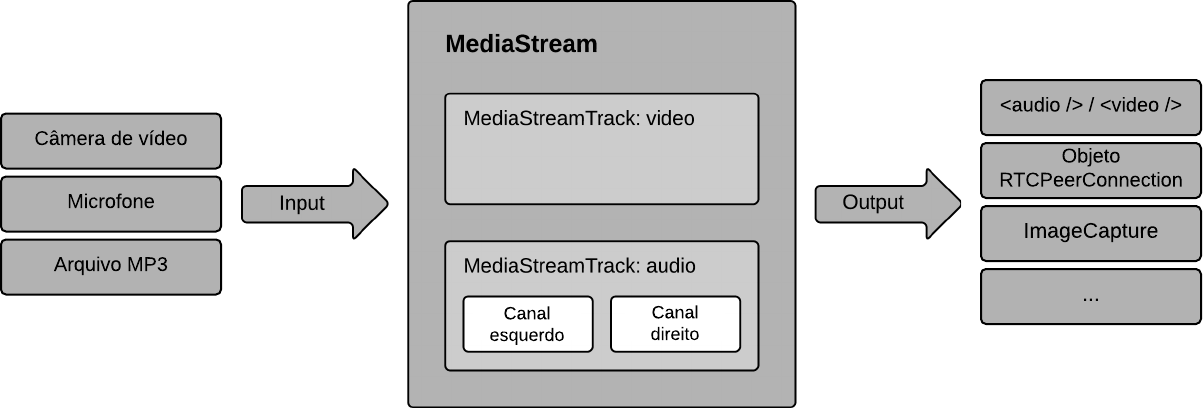
\includegraphics[scale=0.35]{figures/overview-mediastream.png} 
	\caption{Fluxo de dados usando MediaStream}
	\label{fig:overview_mediastream}
\end{figure}

Os chamados consumidores de MediaStream são objetos que conseguem ler o fluxo de dados do \textit{output} dessa interface. A imagem \ref{fig:overview_mediastream} mostra exemplos de saídas existentes. A maior vantagem para o WebRTC é o fluxo poder ser enviado através de objetos RTCPeerConnection, sendo transportado como \textit{streams}, permitindo assim chamadas de áudio e vídeo remotas. Os elementos HTML de áudio e vídeo são responsáveis pela reprodução de mídias no cliente e aceitam saídas MediaStream como entradas de dados.

\subsection{RTCPeerConnection}

De acordo com \cite[Sec.~4.1]{w3cwebrtc2017} é possível realizar conexões ponto-a-ponto entre diferentes computadores em uma rede através de dois objetos RTCPeerConnection. A conexão é realizada através de uma troca de mensagens padronizada por um protocolo de sinalização, similar ao \textit{handshake} do TCP, porém no nível de aplicação. 

Essa troca é chamada de \textit{signaling} e não está definida na especificação, cabendo ao desenvolvedor escolher a maneira de realizá-la. Geralmente é utilizado um servidor que funciona através de WebSockets (no caso desse projeto), requisições HTTP, dentre outros mecanismos.

Em projetos WebRTC executados em uma única aba no navegador não é necessário o uso de um servidor, as informações estão no mesmo contexto de código e conseguimos realizar a conexão sem troca de mensagens através da Internet. Quando alteramos a aplicação para o âmbito da Web, funcionando em produção com \text{peers} remotos, basicamente precisamos de quatro funcionalidades no lado dos servidores:

\begin{itemize}
	\item Tradução de endereço local para público;
    \item Descobrir endereço de IP público do próprio usuário (não do *peer* remoto);
    \item Retransmissão de dados através de servidor reserva caso a conexão ponto-a-ponto não funcione, ou não seja suportada;
    \item Sinalização do cliente enviada para o remoto indicando conexão P2P.
\end{itemize}

Todos esses pontos, exceto o da sinalização, são resolvidos por um protocolo chamado \textit{Interactive Connectivity Establishment} (ICE), que geralmente é utilizado por aplicações WebRTC.

\begin{figure}[ht!]
	\centering
		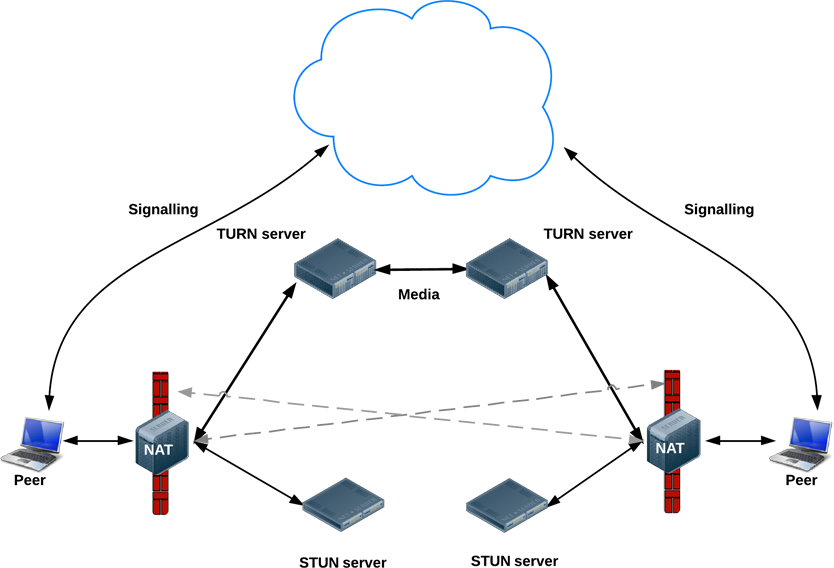
\includegraphics[scale=0.35]{figures/overview-iceprotocol.png} 
	\caption{Protocolo ICE, retirado de \cite{webrtcarchitecture}}
	\label{fig:overview_iceprotocol}
\end{figure}

A figura \ref{fig:overview_iceprotocol} apresenta uma visão geral do processo de \textit{signaling} e seus componentes principais, que são responsáveis cada um por uma  funcionalidade citada acima:

\begin{itemize}
	\item NAT - Responsável por gerar um endereço IP público através de uma tabela \textit{hash} para o cliente;
    \item STUN - Servidor público ou privado, responde com endereço de IP gerado pelo NAT através de uma requisição feita pelo mesmo cliente;
    \item TURN - Servidor responsável por retransmitir os dados caso a conexão ponto-a-ponto não funcione.
\end{itemize}

Com a conexão \textit{peer-to-peer} estabelecida, o servidor deixa de ser necessário e os navegadores estão aptos a transmitir informações em tempo real.

\subsection{RTCDataChannel}

Além de enviar áudio e vídeo, WebRTC tem a capacidade de se comunicar em tempo real por meio da interface RTCDataChannel  usando diversos tipos de dados. 

Essa funcionalidade foi implementada devido a certos casos de uso, como jogos online, transferência de arquivos, documentos de textos colaborativos (por exemplo, Google Docs), dentre outros.

O objetivo é atingir uma baixa latência aliada a uma alta capacidade de transmissão de dados, devido à redução de sobrecarga por \textit{handshakes} TCP e cabeçalhos HTTP. É utilizado o mesmo tipo de conexão para fluxos de áudio e vídeo, através de um objeto RTCPeerConnection. Apesar de muito similar a conexões WebSockets, é mais rápida devido ao fato de estabelecer uma conexão direta de um navegador a outro.

WebRTC é a fundação do sistema de atendimento implementado nesse projeto. A capacidade de comunicação em tempo real, utilização diretamente do navegador e a não necessidade de instalar \textit{plugins} de terceiros, tornaram a ferramenta ideal para solucionar os problemas apresentados no início do trabalho.


% ----------------------------------------------------------
% Trabalhos Relacionados
% ----------------------------------------------------------
\chapter[Trabalhos Relacionados]{Trabalhos Relacionados}\label{chap:relacionados}

Nesta seção serão apresentados projetos relacionados ao tema do presente trabalho. 
Por ser um tema que agrupa dois assuntos, videoconferência e sistema de atendimento ao consumidor, e pela falta de softwares semelhantes, os dois assuntos serão analisados separadamente.

\section{Protocolos para transmissão de vídeo}

\subsection{Protocolo RTMP}

O Protocolo RTMP (\textit{Real-time Messaging Protocol}), desenvolvido pela Macromedia inicialmente como um produto proprietário e de código fechado, foi disponibilizado quando a Adobe adquiriu a empresa e liberou parte da especificação do protocolo

De acordo com sua especificação (\cite{rtpmspec}), o RMTP fornece um serviço bi-direcional de mensagens, tendo como função o \textit{streaming} de áudio, vídeo e dados de alta performance através da Internet. 

O protocolo funciona em cima de serviços de entrega de pacotes confiáveis como TCP, podendo assim ser utilizado sobre HTTP e HTTPS.

Conforme ilustrado na \autoref{fig:overview_rtmp_flash}, o RMTP é responsável por realizar a conexão entre um reprodutor Flash e um servidor de mídia Flash. 

\begin{figure}[ht!]
	\centering
		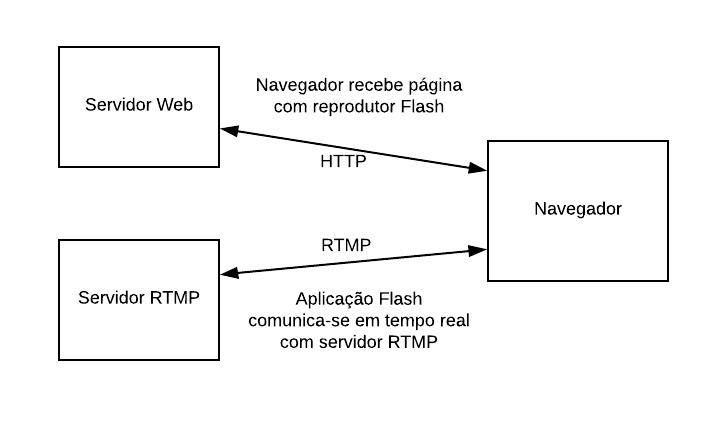
\includegraphics[scale=1]{figures/overview-rtmp-flash.png} 
	\caption{Conexão entre reprodutor e servidor Flash através do RTMP}
	\label{fig:overview_rtmp_flash}
\end{figure}

O reprodutor Flash foi inicialmente desenvolvido para reprodução de animações vetoriais bidimensionais pela Macromedia, mas acabou por tornar-se uma boa escolha para \textit{streaming} de mídia na Internet por sua capacidade de minimizar o tamanho do arquivo, economizando banda e diminuindo a latência.

Somente na versão Flash 10 o suporte a conexões P2P com RTMP foi disponibilizado. 

Há cerca de uma década, o uso do RTMP era uma escolha mais segura no lugar do \textit{WebRTC}, devido ao amplo suporte existente, resultante da presença de \textit{plugins} Flash nos navegadores, além de reprodutores nativos. No entanto, esta situação mudou completamente nos últimos anos. Alguns pontos foram decisivos para a queda do Flash e do RTMP e a ascensão do \textit{WebRTC}:

\begin{itemize}
	\item O código fechado e proprietário do RTMP não agradava certas empresas. Adiciona-se a isso o fato de elas não poderem utilizá-lo sem um reprodutor Flash.
    \item \textit{Plugins} de reprodutores Flash traziam problemas aos navegadores. Os fabricantes de \textit{browsers} começaram a notar diversos gargalos de performance e segurança. Devido à obrigatoriedade do seu uso, surgiram novas frentes para criar tecnologias de \textit{streaming}.
\end{itemize}

Passou-se a buscar uma tecnologia que não obrigasse o usuário a instalar \textit{plugins} no navegador, ou seja, para a qual bastasse o suporte nativo existente.

Não muito tempo depois a Apple removeu o uso do reprodutor Flash nos seus navegadores (presentes em iPhones e iPads) fazendo com que a utilização do protocolo diminuísse. Em 2009 a Apple lançou o HLS (\textit{HTTP Live Streaming}), que será descrito em seguida.

Praticamente ao mesmo tempo a iniciativa de desenvolvimento do HTML5 surgia. A especificação foi apoiada por Steve Jobs, que escreveu uma longa carta \textit{Thoughts on Flash}\footnote{Disponível em: <https://www.apple.com/hotnews/thoughts-on-flash/>. Acesso em 20 mai. 2018.} onde explica a razão de não colocar o reprodutor nos seus aparelhos.

Em questão de performance, as duas tecnologias têm suas vantagens e desvantagens. Foi devido ao modo de uso e a presença delas no dia-a-dia e ao crescente suporte dos navegadores ao \textit{WebRTC} e ao HTML5, que RTMP tornou-se uma opção válida somente para casos específicos de uso.

\subsection{Protocolo HLS}

Protocolo de comunicação implementado pela Apple. Está presente em todos os seus aparelhos e softwares como QuickTime, Safari e iOS.

Funciona sem qualquer configuração adicional em servidores Web convencionais porque realiza todas as suas requisições através de conexões HTTP. Grande vantagem pois é compatível com serviços dedicados a entrega de dados, as chamadas CDN (\textit{Content Delivery Network}).

Sua especificação define uma arquitetura com três componentes principais\footnote{Disponível em: 
<https://developer.apple.com/library/content/documentation/NetworkingInternet/Conceptual/StreamingMediaGuide/HTTPStreamingArchitecture/HTTPStreamingArchitecture.html>. Acesso em 30 mai. 2018.}:


\begin{itemize}
	\item Servidor, responsável por codificar e segmentar o arquivo de mídia.
    \item Distribuidor, um servidor HTTP que responde com a mídia e o arquivo de indexação necessário para reproduzi-la. 
    \item Cliente, reprodutor de mídia com suporte a \textit{streams}.
\end{itemize}

Popular pela qualidade de transmissão, adaptabilidade a diferentes conexões e disponibilidade de serviço. Características existentes devido ao segmentador, componente responsável pela separação da mídia, após a codificação da mesma.

\begin{figure}[ht!]
	\centering
    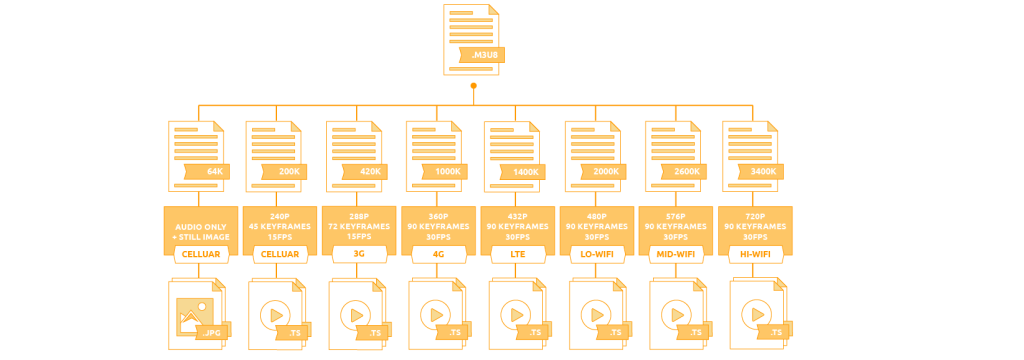
\includegraphics[scale=0.45]{figures/hls-segments.png} 
    \caption{Esquema de segmentação do protocolo HLS.}
    \small Fonte: https://www.encoding.com/http-live-streaming-hls/.
	\label{fig:hls_segments}
\end{figure}

A segmentação, retratada na figura \ref{fig:hls_segments}, compreende a divisão do vídeo em pequenos arquivos \text{TS} de mesma duração. Cada pedaço de mídia separado com sucesso é adicionado a um arquivo com extensão \textit{M3U8}, também chamado de \textit{playlist}. 

As \textit{playlists} são responsáveis por organizar os pedaços de forma sequencial para que o cliente consiga reproduzir a mídia corretamente. Cada \textit{playlist} contém URLs que indicam \textit{playlists} alternativas para diferentes qualidades de conexão. 

Fica então de responsabilidade do reprodutor HLS receber a \textit{playlist} do servidor, escolher a adequada banda larga disponível, agrupar os pedaços de vídeo e reproduzi-los em sequência. 

\section{Sistemas de suporte ao consumidor}

\subsection{Zendesk}

O Zendesk é uma plataforma paga que prove serviços de atendimento ao consumidor aos seus clientes. A plataforma tem o intuito de ajudar empresas a se relacionar melhor com os usuários, criando relações mais significativas\footnote{Disponível em: <https://www.zendesk.com/about>. Acesso em 20 mai. 2018.}. A principio o objetivo é fornecer suporte e melhorar o atendimento, para depois melhorar o relacionamento e o compromisso com o cliente.

\begin{figure}[ht!]
	\centering
		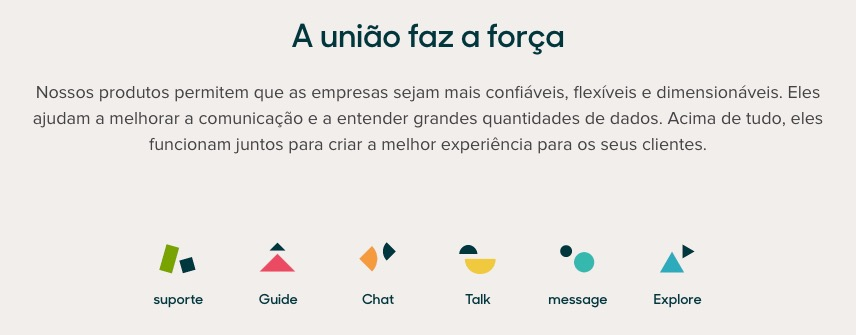
\includegraphics[scale=0.45]{figures/zendesk-modules.jpg} 
	\caption{Módulos disponíveis na plataforma}
	\label{fig:zendesk_modules}
\end{figure}

Composto por diversos módulos, ilustrados na \autoref{fig:zendesk_modules}, o software fornece assistência em diversas áreas: suporte ao cliente; capacitação de atendentes; troca de mensagens; ligações VoIP; e relatórios sobre os atendimentos.

\begin{figure}[ht!]
	\centering
		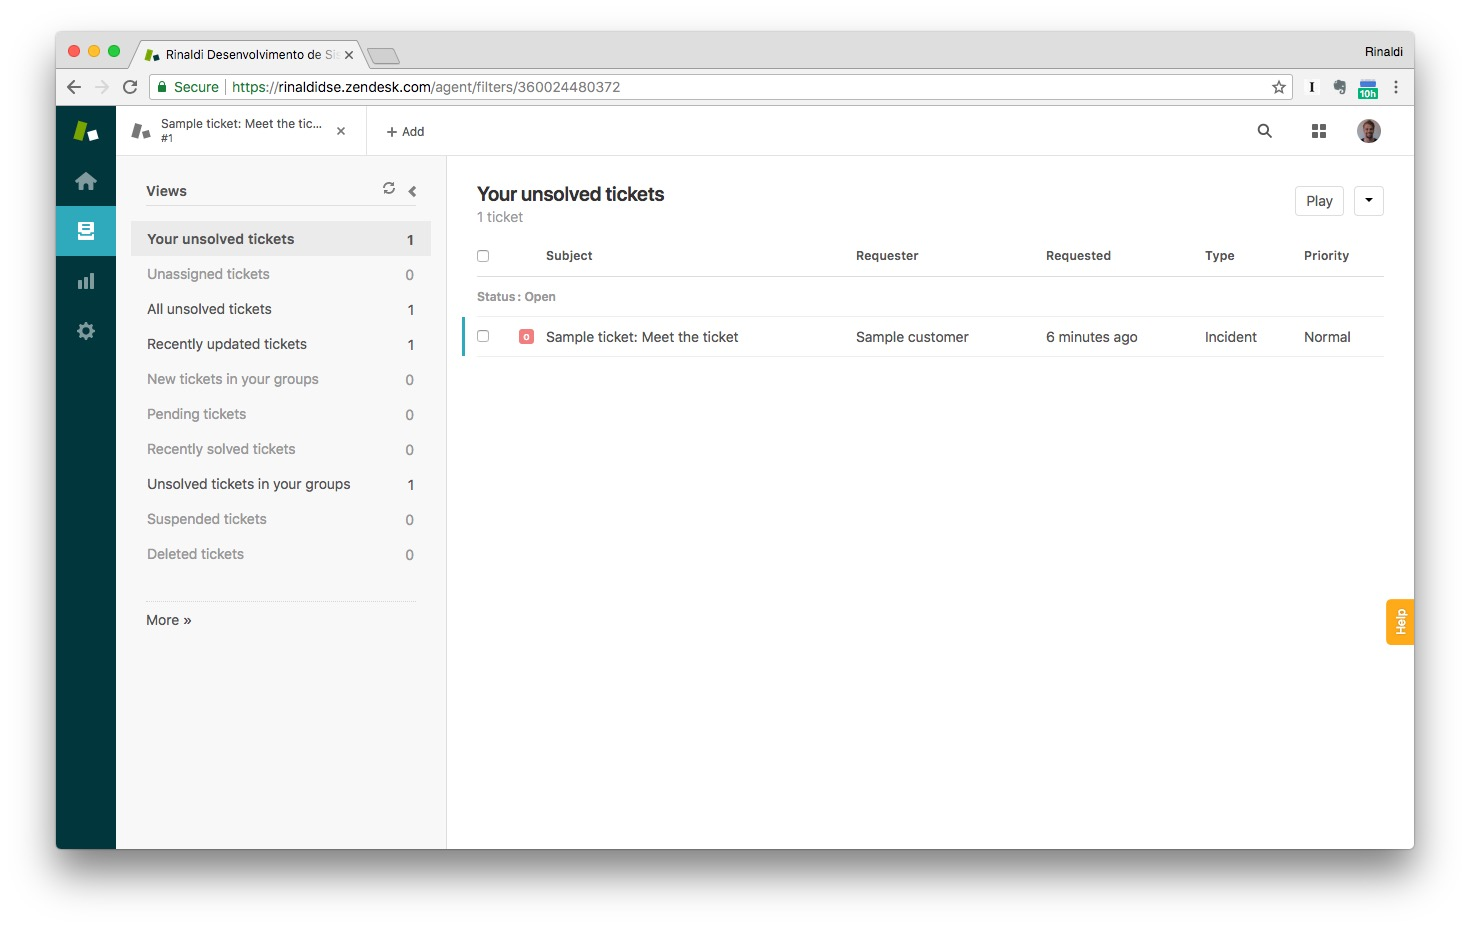
\includegraphics[scale=0.2]{figures/zendesk-ticket-overview.jpg} 
	\caption{Visão geral dos atendimentos}
	\label{fig:zendesk_ticket_overview}
\end{figure}

Atendimentos são chamados de \textit{tickets} dentro da plataforma. Esses contém informações do atendimento, e estão agrupados, sejam pendentes ou resolvidos, em uma só tela de visão geral, mostrada na \autoref{fig:zendesk_ticket_overview}.

\begin{figure}[ht!]
	\centering
		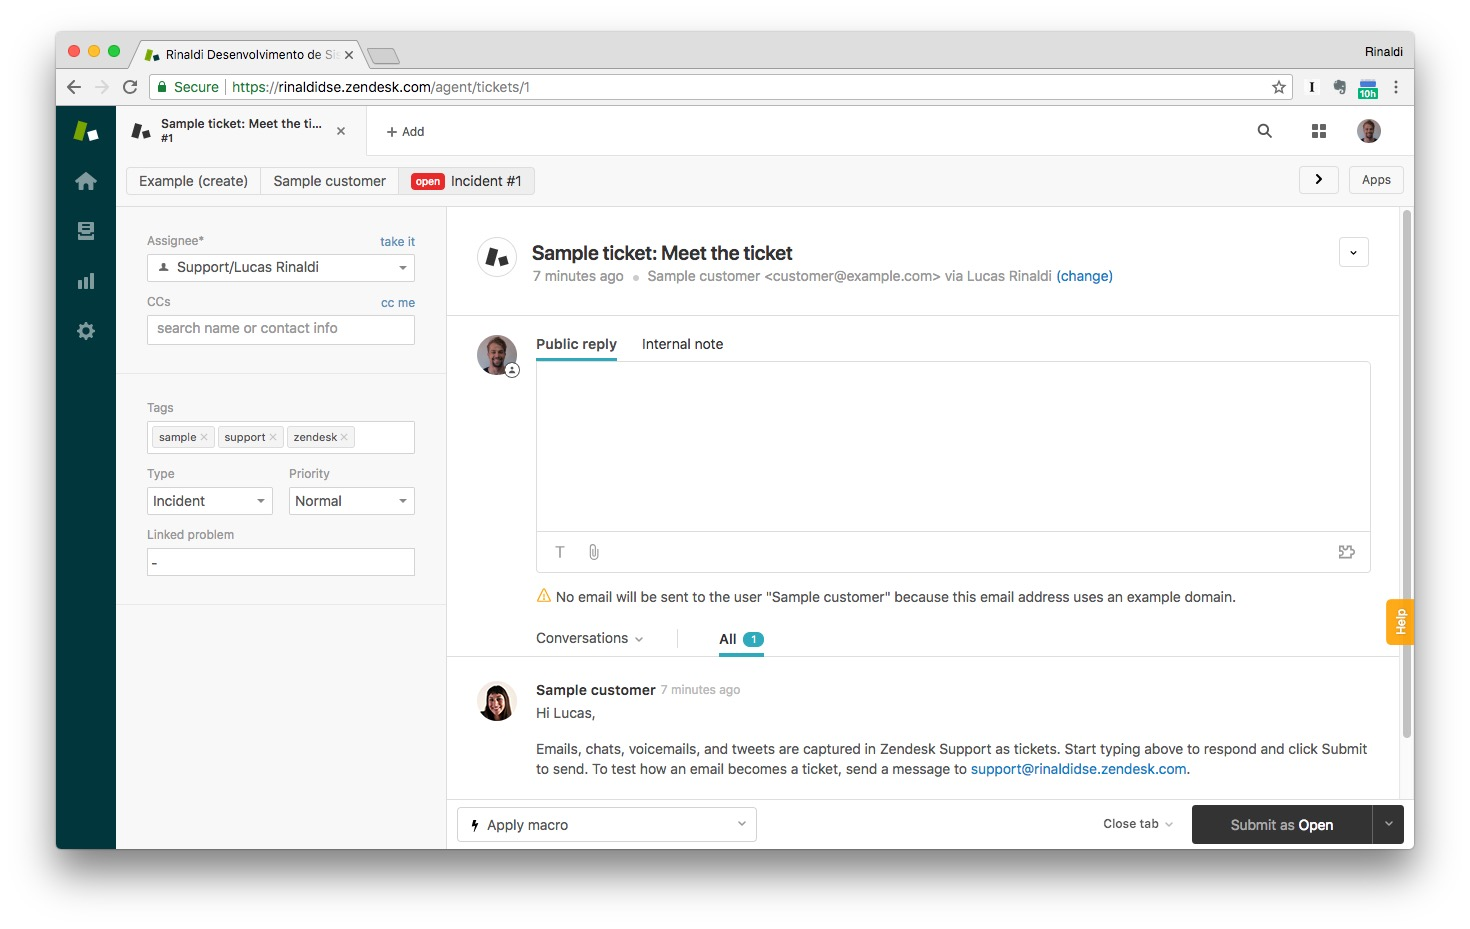
\includegraphics[scale=0.2]{figures/zendesk-ticket.jpg} 
	\caption{Visão interna do atendimento}
	\label{fig:zendesk_ticket}
\end{figure}

Cada \textit{ticket} possui suas próprias características, como prioridade, tipo e área correspondente da empresa (ver \autoref{fig:zendesk_ticket}). O contratante da plataforma pode escolher também por cadastrar um contrato SLA (\textit{Service Level Agreement}) de resolução de problemas, que fica à mostra para que os atendentes não estourem o limite.

Se o cliente necessita de atendimento em tempo real, a empresa pode utilizar um módulo de \textit{live chat}, por meio do qual o cliente entra em contato direto com um atendente designado pela empresa através de uma integração no site da mesma (ver \autoref{fig:zendesk_chat}).

\begin{figure}[ht!]
	\centering
		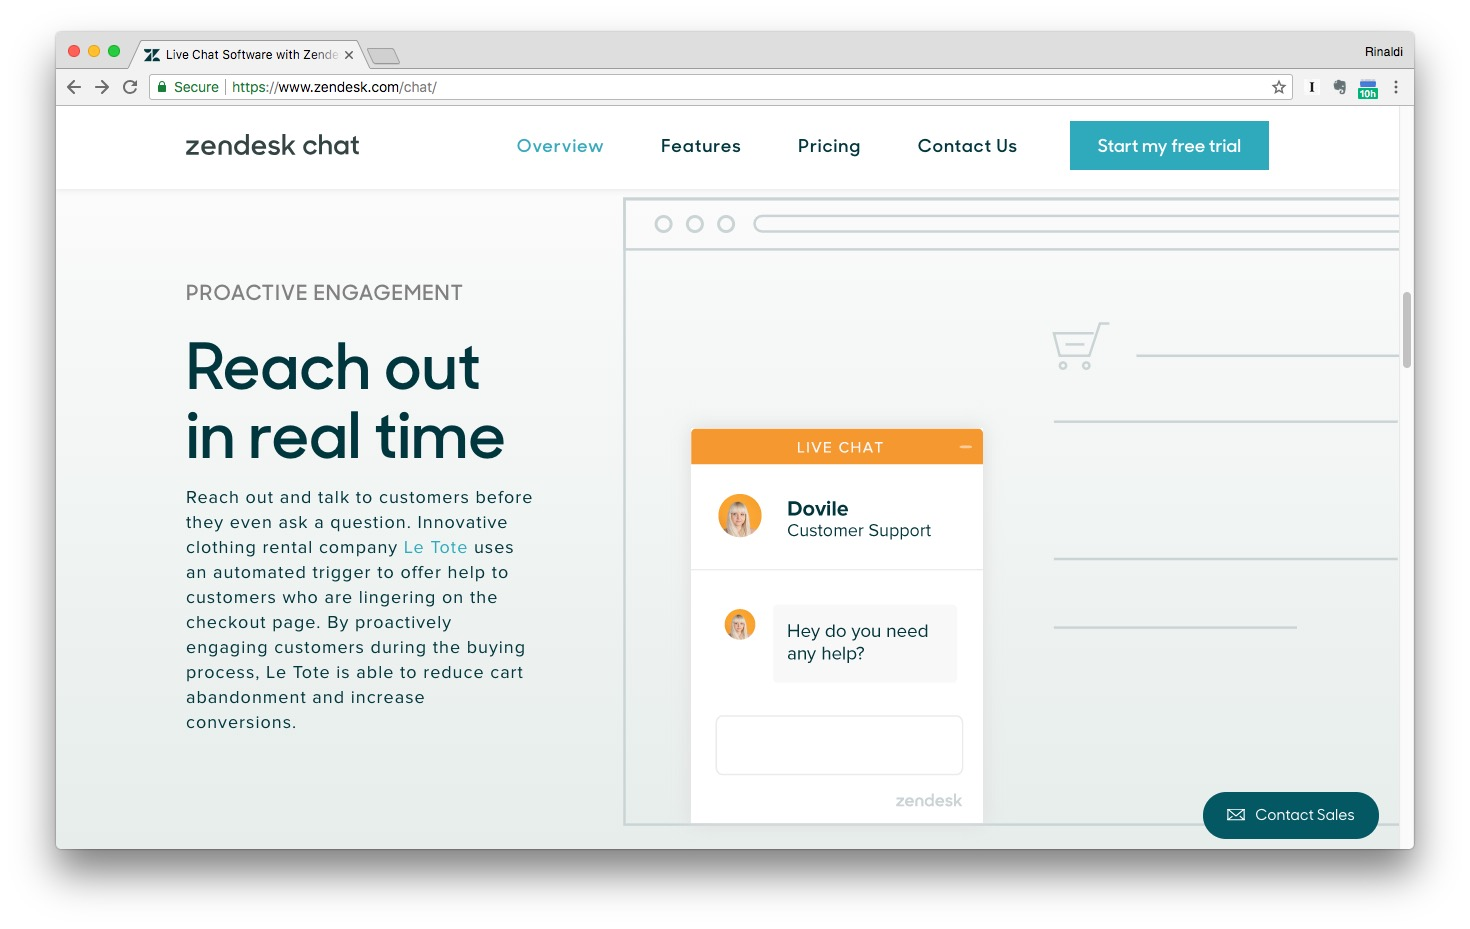
\includegraphics[scale=0.2]{figures/zendesk-chat.jpg} 
	\caption{Integração de chat no site do cliente}
	\label{fig:zendesk_chat}
\end{figure}

Apesar de esse atendimento acontecer somente por meio de troca de mensagens, outro módulo funciona com VoIP, porém não existem chamadas por vídeo.

Muito utilizado, Zendesk está presente em diversas \textit{startups} e grandes empresas, como AirBnB e OLX. Podemos ver mais exemplos na sua página de clientes\footnote{Disponível em: <https://www.zendesk.com/why-zendesk/customers>. Acesso em 20 mai. 2018.}.  A plataforma serviu de base para as primeiras ideias do projeto.
%FRANK: só é usado por startups? grandes empresas não usam?
%LUCAS: Adicionei e com referencias 

\subsection{Intercom}

Bastante voltada para soluções que colocam a troca de mensagens em foco\footnote{Disponível em: <https://www.intercom.com/about>. Acesso em 30 jun. 2017.}. Intercom possui múltiplos produtos que resolvem diferentes problemas nas empresas, todos com o objetivo de oferecer suporte e ajudar seus usuários diretos a reterem clientes.

O modelo de múltiplos produtos dá ao cliente oportunidade de escolher cada um separadamente. São eles \textit{Messenger}, \textit{Inbox} e \textit{Articles}.

%FRANK: essa figura não traz nenhuma informação técnica sobre o produto, não me parece apropriada para um TCC, serve só para marketing
\begin{figure}[ht!]
	\centering
		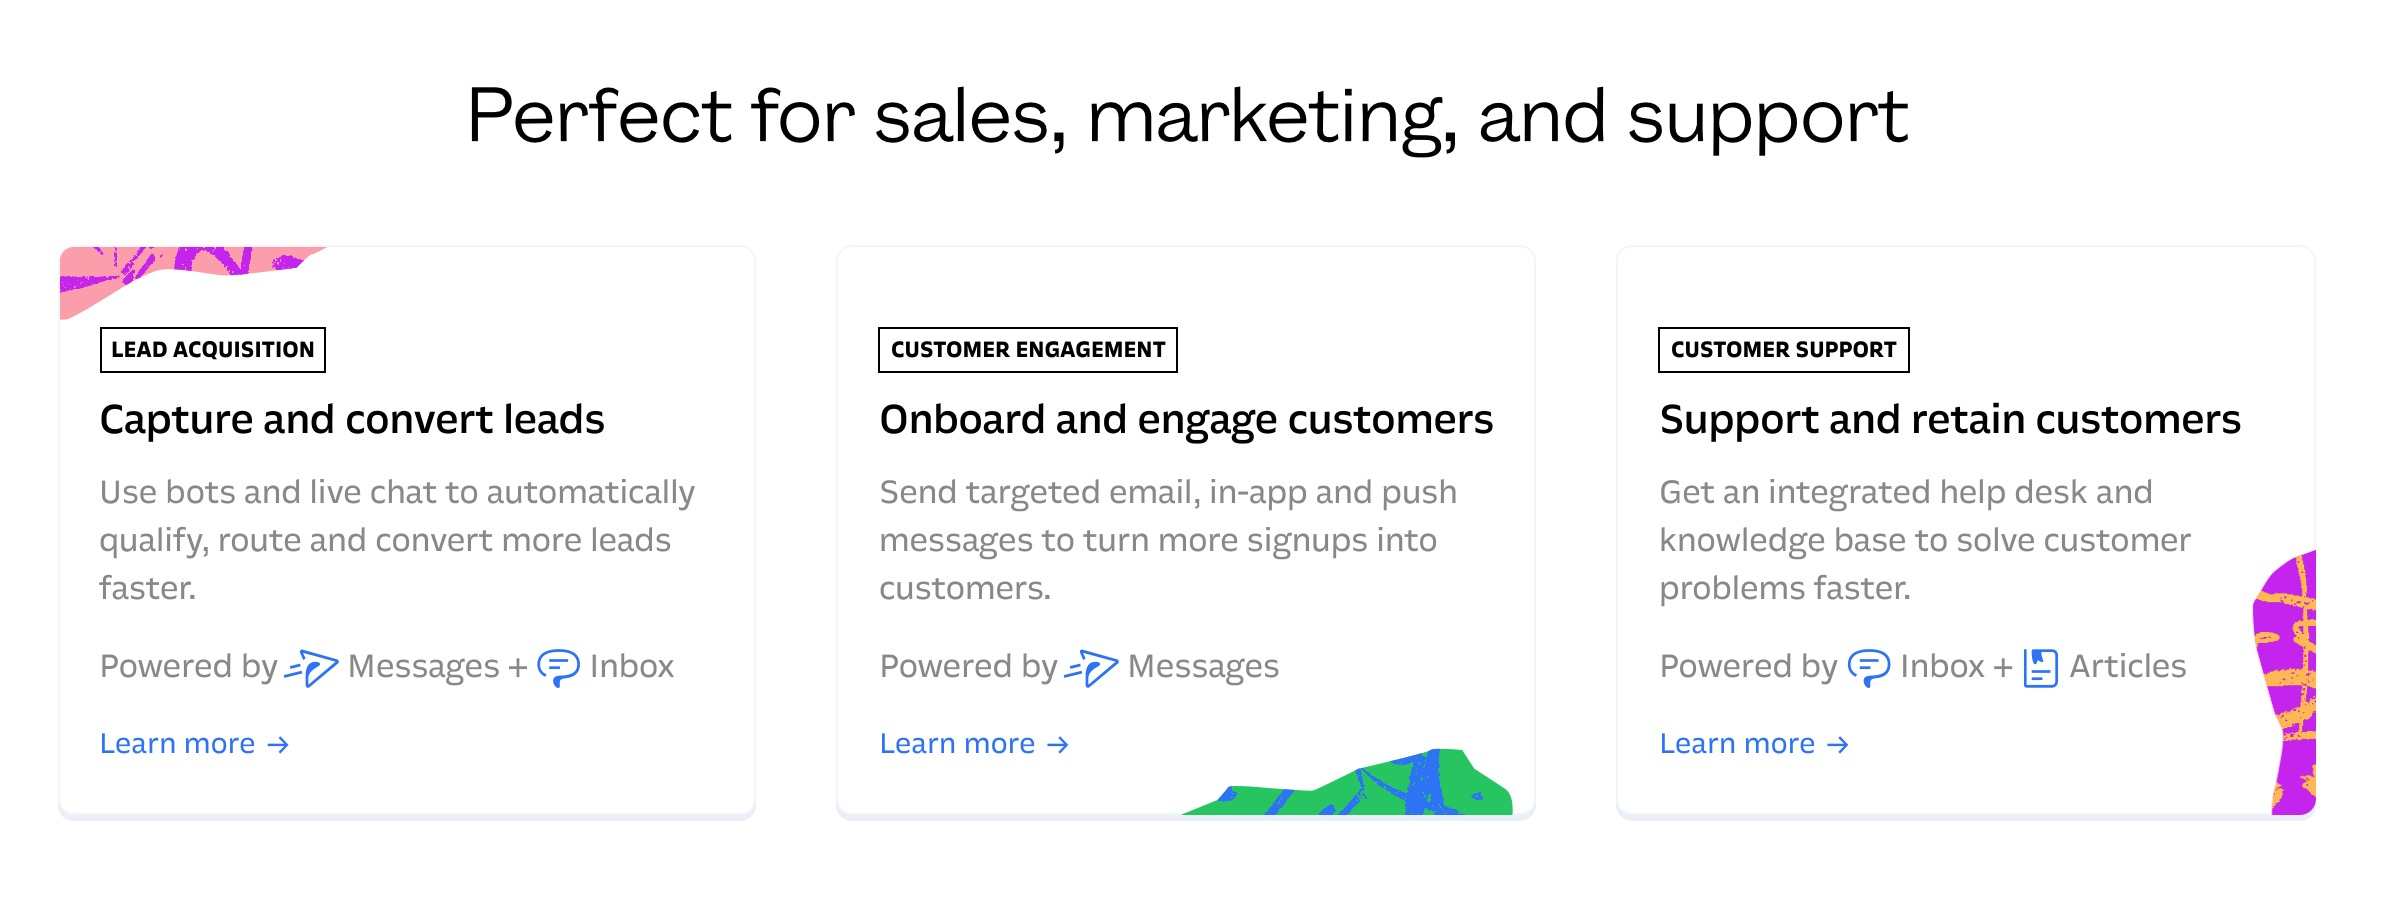
\includegraphics[scale=0.2]{figures/intercom-use-cases.jpg} 
	\caption{Produtos e casos de uso do Intercom}
	\label{fig:intercom_use_cases}
\end{figure}

Além da liberdade, podemos ver em \autoref{fig:intercom_use_cases} as sugestões de combinações dentro da plataforma para cada especifico caso de uso de acordo com a sua necessidade.

Nota-se que diferentemente do Zendesk, a empresa direciona grande parte de seus esforços a área de retenção de clientes. Coloca-os em etapas de funil de vendas e utilizando o seu produto \textit{Messenger} envia mensagens de acordo com a etapa atual. No projeto apresentado nesse trabalho não temos um foco em marketing ou vendas, por isso a pequena explicação.

Como citado acima, seus produtos prezam pela troca de mensagens. O módulo \textit{Inbox} funciona como um \text{live chat} integrado no site do usuário, conectando assim o seu cliente com atendentes de suporte.

\begin{figure}[ht!]
	\centering
		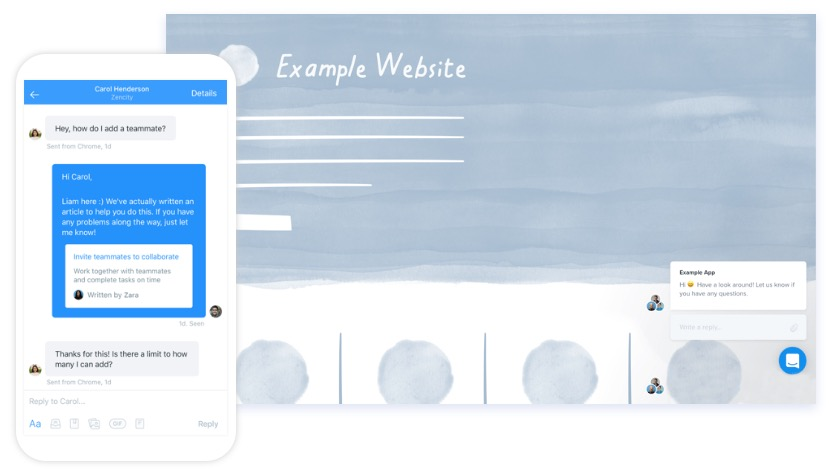
\includegraphics[scale=0.4]{figures/intercom-inbox.jpg} 
	\caption{Intercom Inbox}
	\label{fig:intercom_inbox}
\end{figure}

Sua vantagem é possuir um conexão facilitada com \textit{Articles}, seu outro produto, e assim fazer com que o atendente resolva os problemas de forma rápida e fácil.

\textit{Articles} é uma central de ajuda, onde guias sobre o \textit{software} e perguntas mais frequentes podem ser publicadas para melhor resolução de problemas. 

\begin{figure}[ht!]
	\centering 
		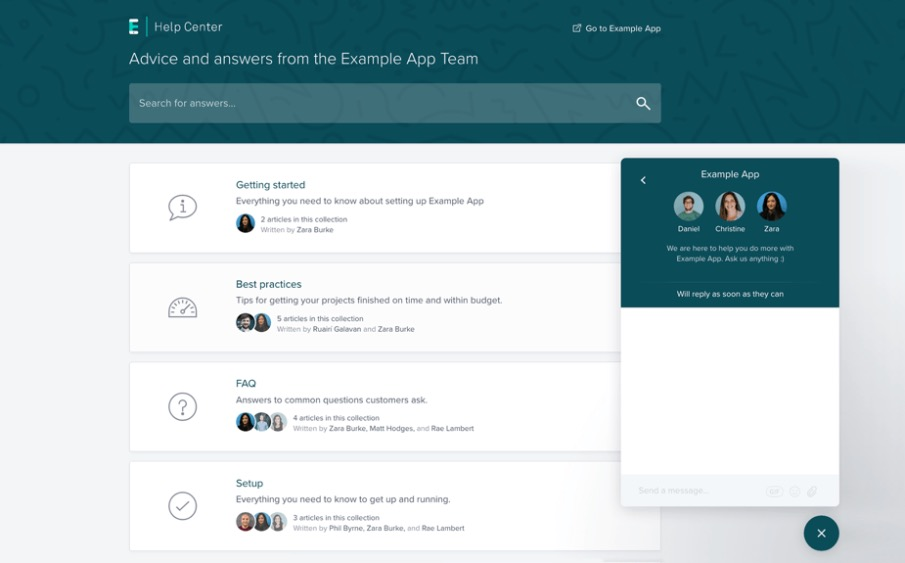
\includegraphics[scale=0.4]{figures/intercom-articles.jpg} 
	\caption{Intercom Articles}
	\label{fig:intercom_articles}
\end{figure}

A integração com o \textit{Inbox} serve para que o seu time consiga escalar o suporte. No momento que o atendente recebe uma palavra-chave a central de ajuda retorna uma lista de artigos relacionados à mesma. 

Traz também relatórios e ações sobre como os clientes estão utilizando a central e como melhora-lá. Na \autoref{fig:intercom_articles_actions} vemos exemplos de ações a serem tomadas.

\begin{figure}[ht!]
	\centering 
		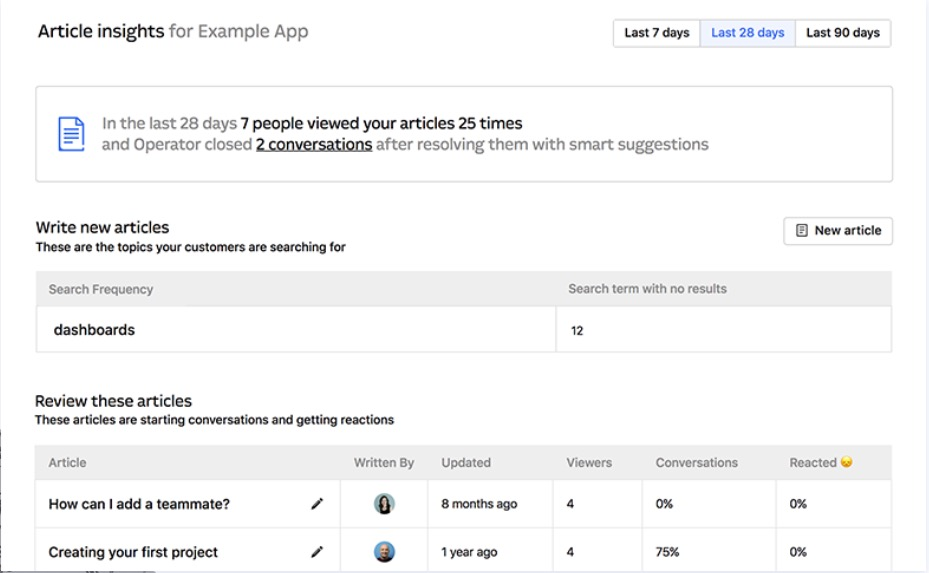
\includegraphics[scale=0.4]{figures/intercom-articles-actions.jpg} 
	\caption{Relatório e ações no Intercom Articles}
	\label{fig:intercom_articles_actions}
\end{figure}

Centrado e com produtos voltados para o marketing algumas funcionalidades divergem do objetivo desse projeto, porém o Intercom serviu de inspiração para ideias futuras. 

A integração da central de ajuda dentro do chat é um recurso poderoso que poderia ser integrado dentro de uma videoconferência. Em tempo real o atendente pode pesquisar sobre o assunto que o cliente está falando e indicar a resposta certa, facilitando a resolução do problema.


% ----------------------------------------------------------
% Projeto
% ----------------------------------------------------------
\chapter[Projeto de implementação]{Projeto de implementação}\label{chap:projeto}

%FRANK: Adicionar parágrafo introdutório, descrevendo de forma sucinta o conteúdo do capítulo. 

\section{Análise de Requisitos}

Dois tipos de requisitos foram levantados para a implementação do projeto: Requisitos Funcionais (RF), que são aqueles que definem as funcionalidades e como o \textit{software} se comporta; e os Requisitos Não-Funcionais (RNF), que são responsáveis por especificar quesitos mais técnicos do \textit{software}, como tecnologias, segurança e desempenho. 

Para definição dos RF, foram analisados programas no estado da arte das duas categorias abordadas (videoconferência e atendimento ao consumidor) e coletadas funcionalidades consideradas importantes. Os RNF foram definidos a partir de estudos de aplicações Web modernas, com exceção do WebRTC que foi definido desde o principio. Requisitos funcionais serão apresentados com um diagrama de casos de uso, sendo cada caso um requisito. 

Os RF levantados são representados como casos de uso na \autoref{fig:usecases}.

\begin{figure}[ht!]
	\centering
    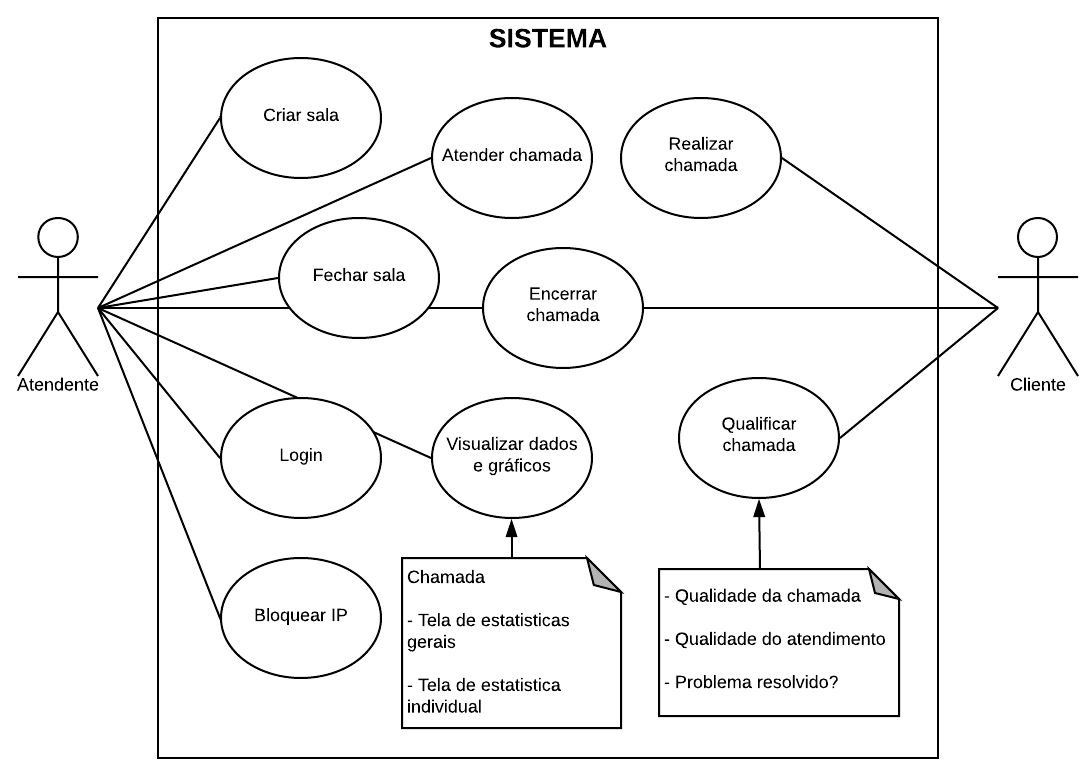
\includegraphics[scale=0.4]{figures/usecases.png} 
	\caption{Requisitos Funcionais do sistema representados por casos de uso}
	\label{fig:usecases}
\end{figure}
%FRANK: Aumentar tamanho da figura para que fique legível

Os RNF levantados são os seguintes:
\begin{itemize}
	\item RNF 01: Utilizar a linguagem JavaScript.
    \item RNF 02: Arquitetura REST para API.
    \item RNF 03: Arquitetura com WebSockets para estabelecer a conexão P2P.
    \item RNF 04: Utilizar plataforma NodeJS para o servidor.
    \item RNF 05: Utilizar \textit{framework} ExpressJS para API.
    \item RNF 06: Utilizar \textit{framework} SocketIO para suporte a WebSocket.
    \item RNF 07: Utilizar \textit{framework} ReactJS para renderizar interface no navegador.
    \item RNF 08: Utilizar PostgreSQL como gerenciador de banco de dados.
    \item RNF 09: Suporte a dispositivos móveis.
    \item RNF 10: Utilização de WebRTC para videoconferência.
%FRANK: Adicionar requisitos sobre qualidade da comunicação (limite de retardo, qualidade de áudio e vídeo, poucas quedas de conexão)
\end{itemize}

\section{Protótipos de tela}

\subsection{Login}

A tela inicial da aplicação é a de login, constituída de um pequeno formulário de autenticação e um logo no canto esquerdo. 

Como nenhum cliente necessita de cadastro para realizar chamadas, a tela está disponível somente para os atendentes entrarem no gerenciamento de tickets. 

 Ao inserir os dados corretamente o atendente é redirecionado para a lista de tickets.
 %(ref lista de tickets) 
 Caso contrário, um erro é mostrado no formulário.

% Protótipo da telas de login

\subsection{Gerenciamento de tickets}

A tela de Gerenciamento de Tickets é a primeira tela do sistema de atendimento. Podemos observar na figura 
%(protótipo!!!) 
que a interface é constituída de uma barra lateral na esquerda e o conteúdo principal à direita. 

O conteúdo a ser mostrado na direita dependerá do contexto da aplicação e de onde o usuário está no momento. Temos três situações diferentes que podem acontecer.

De inicio, temos a tela de estatísticas de tickets relacionados ao atendente (\autoref{fig:support_statistics}). Essa tela aparece no conteúdo principal quando o usuário não tem nenhum ticket selecionado. Ela reune informações de todos os atendimentos feitos pelo usuário autenticado, como:

\begin{itemize}
  \item Número total de chamadas;
  \item Tempo total de chamada;
  \item Média de qualidade de atendimento;
  \item Média de qualidade de ligação; e
  \item Porcentagem de problemas resolvidos.
\end{itemize}

\begin{figure}[ht!]
	\centering
    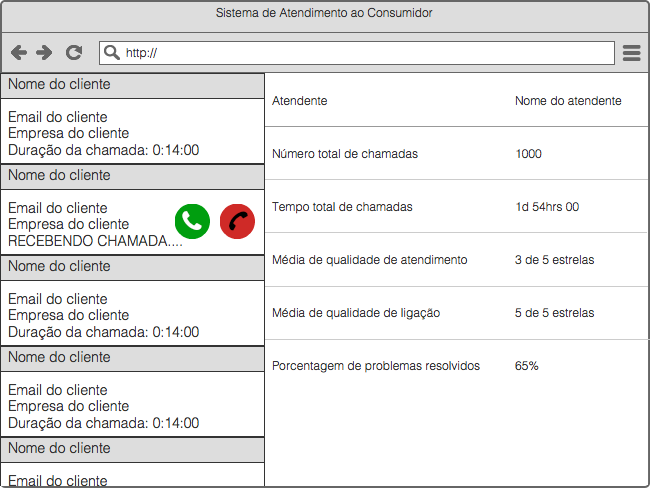
\includegraphics[scale=0.4]{figures/support-statistics.png} 
	\caption{Tela de estatísticas do atendente}
	\label{fig:support_statistics}
\end{figure}

A segunda tela (\autoref{fig:ticket_statistics}) diz respeito a informações sobre um ticket específico que está selecionado. É importante frisar que o item selecionado é de um atendimento já encerrado, pois o conteúdo é diferente. 
%FRANK: explicar quais são essas diferenças
Os dados presentes são:

\begin{itemize}
  \item Nome do cliente e e-mail do cliente;
  \item Empresa, se existir;
  \item Descrição do problema;
  \item Duração do atendimento;
  \item Qualidade da ligação;
  \item Qualidade do atendimento; e se
  \item O problema foi resolvido.
\end{itemize}

\begin{figure}[ht!]
	\centering
    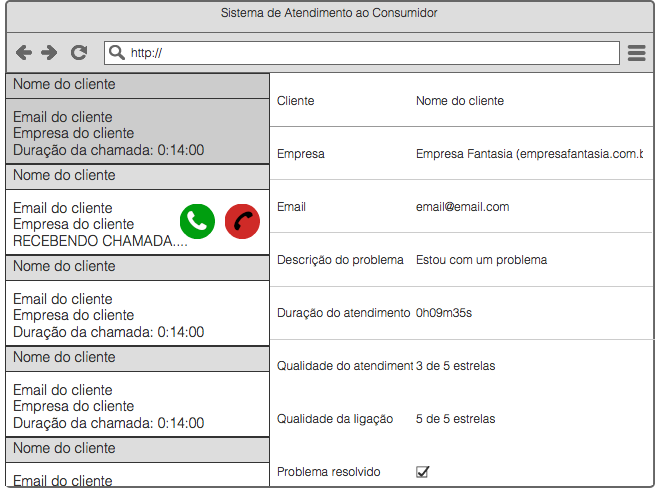
\includegraphics[scale=0.4]{figures/ticket-statistics.png} 
	\caption{Tela de estatísticas de um ticket encerrado}
	\label{fig:ticket_statistics}
\end{figure}

Por último, temos na \autoref{fig:call_statistics} a tela que mostra o conteúdo de um ticket em aberto, ou seja, que o cliente está requisitando a chamada no momento. Nessa tela são exibidas as seguintes informações:

\begin{itemize}
	\item Nome do cliente e email do cliente;
    \item Empresa, se existir;
    \item Descrição do problema; e
    \item Botões de aceitar ou recusar chamada.
\end{itemize}

\begin{figure}[ht!]
	\centering
    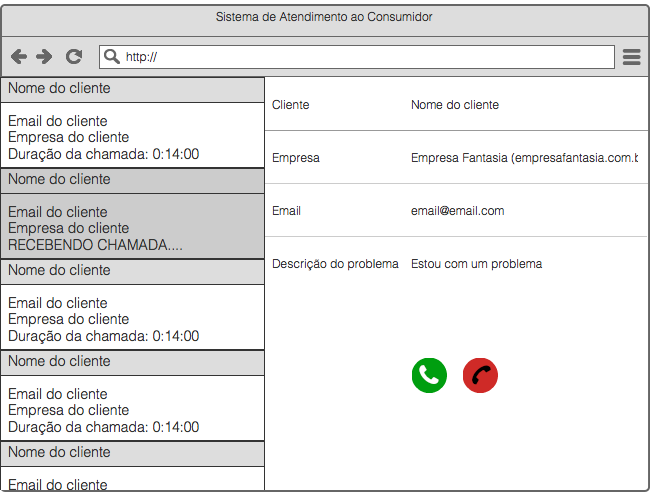
\includegraphics[scale=0.4]{figures/call-statistics.png} 
	\caption{Tela de estatísticas de uma requisição de chamado}
	\label{fig:call_statistics}
\end{figure}

\subsection{Plugin para videoconferência}

O sistema de atendimento fornece aos seus usuários uma maneira de integrar um videochat no site da empresa através de um plugin. Esse plugin é feito a partir de tecnologias disponíveis no navegador (ou seja, não requer outros plugins, como Flash). O chat fornece três interfaces diferentes:

\begin{itemize}
  \item Plugin fechado e com um botão para abrir localizado no canto direito inferior;
  \item Plugin aberto com um formulário de requisição de atendimento; e
  \item Plugin aberto após encerramento de chamada com botões para qualificar atendimento.
\end{itemize}

\subsection{Tela de videoconferência}

Consiste na interface que compreende a funcionalidade principal do sistema de atendimento. Foi separada em um módulo e está presente tanto na aplicação voltada para atendentes quando no videochat integrado no site do cliente. A tela contém os seguintes itens:

\begin{itemize}
 \item Imagem da câmera do cliente sendo atendido;
 \item Imagem da câmera do atendente prestando atendimento;
 \item Botões para encerrar chamada e silenciar microfone;
 \item Dados sobre o presente atendimento.
\end{itemize}

\begin{figure}[ht!]
	\centering
    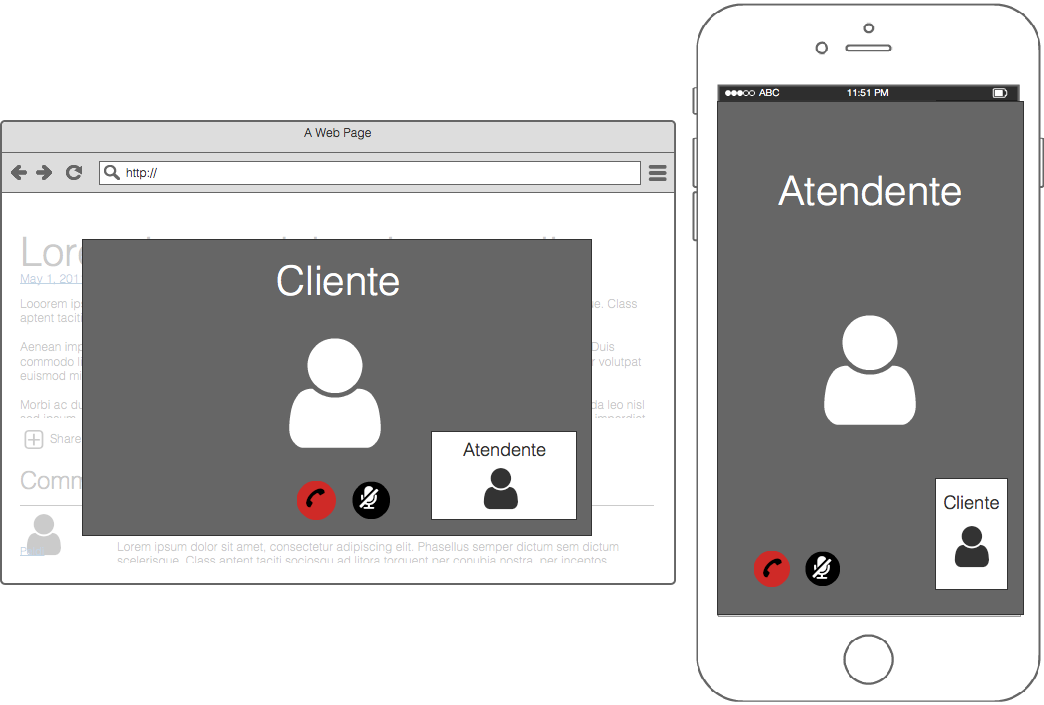
\includegraphics[scale=0.2]{figures/videoconference.png} 
	\caption{Videoconferência entre atendente e cliente}
	\label{fig:videoconference}
\end{figure}

\section{Arquitetura}

Observamos na \autoref{fig:overview_architecture} uma visão geral da arquitetura do sistema. Notamos que o modelo utilizado é o clássico cliente-servidor.

\begin{figure}[ht!]
	\centering
		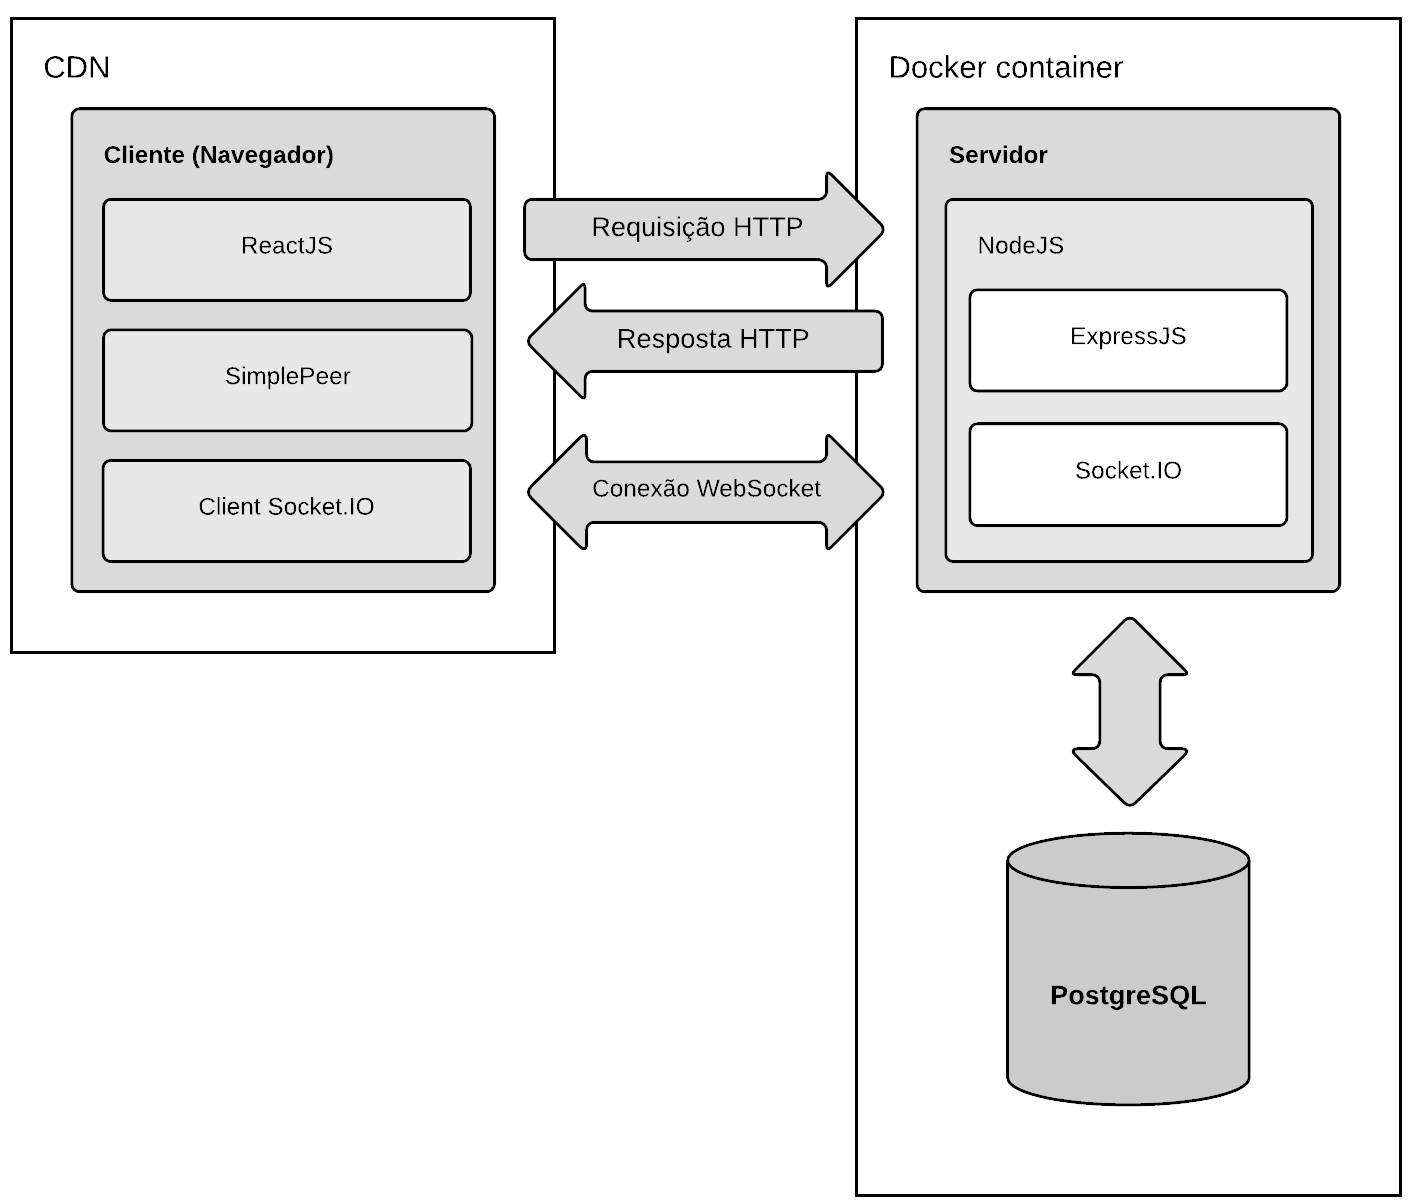
\includegraphics[scale=0.2]{figures/overview-architecture.png} 
	\caption{Arquitetura do sistema}
	\label{fig:overview_architecture}
\end{figure}

\subsection{Servidor}

Todo o \textit{back-end} foi implementado sobre a plataforma NodeJS. Essa tornou-se popular dentre os desenvolvedores nos últimos tempos devido à capacidade de executar código JavaScript fora do navegador. 

Podemos elencar três componentes mais importantes no lado do servidor. O primeiro deles é a base, uma interface de programação de aplicação (API) nos modelos da arquitetura REST, implementada com o \textit{framework} ExpressJS, utilizado para facilitar a construção de aplicações Web. O servidor da API, além de ser utilizado para salvar informações no banco de dados, também é responsável por iniciar a conexão através de \textit{sockets}.

O segundo componente é outro \textit{framework}, SocketIO, desenvolvido com o o objetivo de facilitar o \textit{upgrade} de requisições HTTP e estabelecer a comunicação através de WebSockets. Esse \textit{framework} abstrai as APIs complexas do navegador em padrões já conhecidos, fornecendo ao desenvolvedor uma outra arquitetura mais simples de usar.

Por último, temos o gerenciador de banco de dados PostgreSQL, que armazena os dados das chamadas, atendentes, administradores e clientes do sistema.

\subsection{Cliente}

O lado do cliente será sempre executado em um navegador, ou seja, foi inteiramente implementado com HTML e JavaScript. 

Utiliza o \textit{framework} React para renderizar interfaces. É baseado em composição de componentes, sendo cada um deles uma peça da interface. Esses componentes têm acesso às APIs nativas do navegador, podendo assim realizar requisições HTTP através de interfaces como AJAX.

É responsabilidade do cliente solicitar uma conexão \text{peer-to-peer} com um navegador remoto, conforme ilustrado na figura \ref{fig:peer_connection}, que remete a assuntos abordados no capítulo \ref{chap:fundamentacao}.

\begin{figure}[ht!]
	\centering
		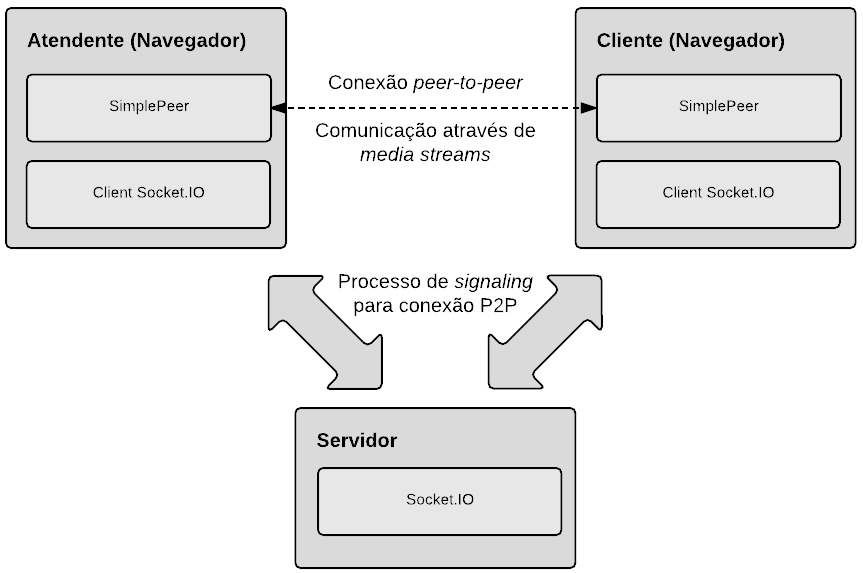
\includegraphics[scale=0.35]{figures/overview-client.png} 
	\caption{Conexão peer-to-peer através de WebSockets}
	\label{fig:peer_connection}
\end{figure}

Com a conexão estabelecida entre os dois pontos, a aplicação renderiza automaticamente uma nova tela, na qual o cliente consegue enxergar o atendente e vice-versa.

\section{Modelagem do banco de dados}

O diagrama de entidades representado na figura \ref{fig:database_model}, contém três modelagens que representam a aplicação. 

\begin{figure}[ht!]
	\centering
		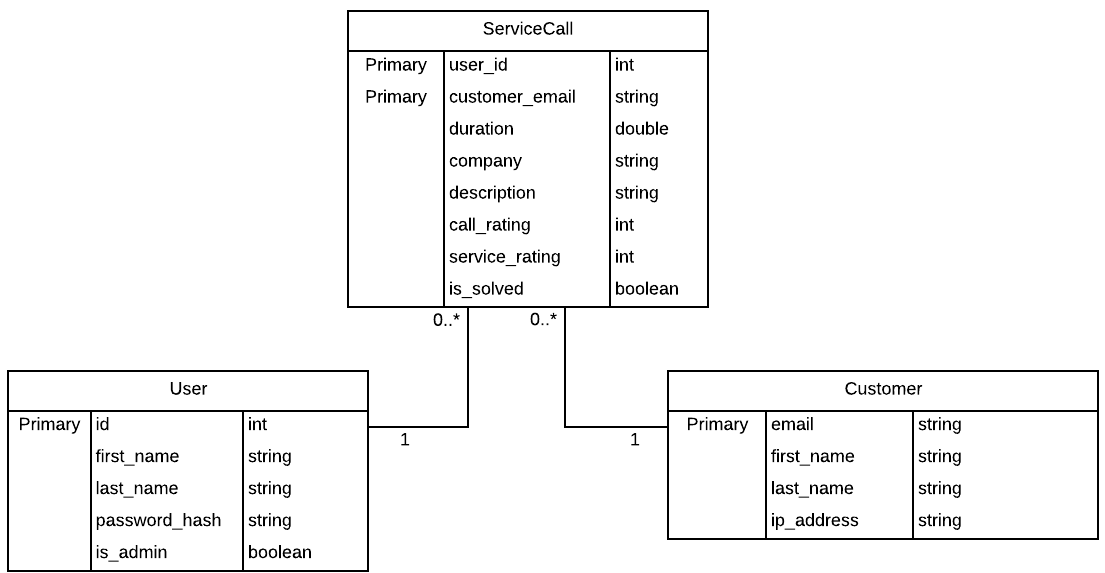
\includegraphics[scale=0.8]{figures/database-model.png} 
	\caption{Entidades do banco de dados}
	\label{fig:database_model}
\end{figure}

A entidade \textit{User} representa os atendentes do serviço de atendimento ao consumidor. Todo atendente necessita fazer login no sistema para poder criar salas e atender clientes. Esse mesmo usuário tem permissão para visualizar dados e estatísticas de chamadas.

Para representar os clientes que realizam chamadas de suporte criamos a entidade \textit{Customer}. Essa entidade não necessita de login para solicitar um atendente, visto que o objetivo do sistema é prover uma maneira fácil para pessoas obterem resolução de problemas.

Por fim, as chamadas de suporte são representadas pela entidade \textit{ServiceCall}. Essa entidade possuí o tempo de duração de atendimento e faz a relação entre atendente e consumidor. Foram adicionados também dados da chamada, como avaliação e se o problema foi resolvido ou não, para que seja possível registrar estatísticas e criar uma página com informações para os atendentes.


% ----------------------------------------------------------
% Implementação
% ----------------------------------------------------------
\chapter[Implementação]{Implementação}\label{chap:implementacao}

\section{Tecnologias e ferramentas}

\subsection{JavaScript}

No início da Internet, os únicos documentos transferidos eram páginas estáticas HTML. Nenhuma página possuía conteúdo dinâmico e nem possibilidade de interação com a mesma. Javascript foi idealizado com esse intuito. Desenvolver uma forma com que os usuários possam realizar ações e receber resultado de forma mais rápida. A web precisava ser mais dinâmica, de acordo com Marc Andressen, fundador da Netscape Communications\footnote{Disponível em: <https://auth0.com/blog/a-brief-history-of-javascript/>. Acesso em 20 mai. 2018.}.

Criada em 1995, no meio da chamada \textit{browsers war} (ou guerra dos navegadores). Foi desenvolvida em apenas dez dias por Brendan Eich, e a princípio levou o nome \textit{Mocha}. Em agosto do mesmo ano, a Netscape em parceria com a Sun Microsystems (criadora da linguagem Java, posteriormente adquirida pela Oracle) apresentou o  Javascript\footnote{Disponível em: <http://tech-insider.org/java/research/1995/1204.html>. Acesso em 20 mai. 2018.}, com o intuito de torná-la a linguagem de script oficial dos navegadores.

Javascript na verdade é uma implementação/extensão da especificação ECMAScript (\cite{ecmascript}), desenhada para facilitar a padronização de  linguagens proprietárias baseadas na ECMAScript, como por exemplo JScript, a linguagem de script da Microsoft. Essa especificação define uma linguagem com paradigma orientado a objetos, tipagem fraca e que funciona através de interpretadores, ou seja, não compilada (diferentemente de Java, apesar do nome).

A grande diferença entre a especificação e a implementação são as interfaces de aplicação disponíveis na linguagem executada pelos navegadores. Como por exemplo, a API voltada para interação com HTML, chamada de DOM ou \textit{Document Object Model}, que foi a primeira responsável pelo maior dinamismo das páginas da Internet. Hoje em dia temos interfaces para captura de mídia (áudio, vídeo); interação com dispositivos móveis (bateria, GPS); e até para conexões \textit{peer-to-peer}, assunto do presente trabalho.

Cada vez mais utilizada devido a sua presença na Web, muitos desenvolvedores acreditaram que a linguagem era digna de funcionar também no servidor, eliminando a necessidade de navegadores. Com o lançamento da \textit{engine} V8, o interpretador desenvolvido pela Google para ser utilizado no seu navegador Chrome, a linguagem atingiu um outro nível de utilização, passando a ser utilizada também em servidores, através do ambiente Node.js. Denominado \textit{cross platform}, o Node.js é capaz de ser executado em qualquer sistema operacional e funciona em cima do interpretador V8, tornando a linguagem livre das amarras dos navegadores. A linguagem também pode ser encontrada em aplicações de banco de dados não-relacionais, como o MongoDB.

Nesse projeto, Javascript será utilizado tanto no cliente como no servidor (com exceção do banco de dados). Devido a isso, o primeiro item do tópico de tecnologias foi uma introdução à mesma. Abordaremos nos próximos itens como esta linguagem será utilizada no projeto.

\subsection{Servidor}
%FRANK: Essa subseção ficou confusa. Mistura a tua proposta com tecnologias utilizadas. Sugiro separar bem essas duas coisas.
%LUCAS: Movi a subseção de projeto para implementação

Servidor constituído de uma API e uma conexão com WebSockets. A interface REST servirá para enviar e receber dados de sobre os atendimentos do banco de dados. Utilizaremos WebSockets para realizar as conexões P2P nas videoconferências.

Composto por \textit{frameworks} e bibliotecas desenvolvidos com a plataforma NodeJS. Utiliza o gerenciador de pacotes NPM ou \textit{Node Package Manager} para instalação das dependências do projeto.

ExpressJS é a ferramenta utilizada para criação da API REST que servirá para enviar e receber dados sobre os atendimentos do banco de dados. Responsável também por devolver uma página HTML a ser integrada no cliente.

SocketIO fornece uma interface de aplicação em cima de uma conexão por WebSockets e auxiliará as conexões \textit{peer-to-peer}.

E por final possui uma biblioteca, chamada ObjectionJS. Funciona como um ORM ou \textit{Object Relational Mapping}, tornando mais fáceis as operações no banco de dados.

\subsubsection{ExpressJS}

Um dos primeiros e mais famosos \textit{frameworks} desenvolvidos para servir aplicações Web com NodeJS. Tornou-se popular pela sua facilidade de uso, alta possibilidade de customização e suporte a ferramentas de linha de comando. Observamos em seu site\footnote{Disponível em: <http://expressjs.com/>. Acesso em 15 mai. 2018.} o foco em se manter como uma ferramenta minimalista e \textit{unopinionated}, que tem como objetivo dar mais controle aos desenvolvedores, diferentemente de grandes \textit{frameworks} como Ruby On Rails.

Possui uma arquitetura voltada a \textit{middlewares}\footnote{Disponível em: <https://www.cleveroad.com/blog/the-best-node-js-framework-for-your-project--express-js--koa-js-or-sails-js>. Acesso em 20 mai. 2018.}. Esse tipo de arquitetura suporta o registro de módulos que são executados em ordem a cada ciclo de requisição e resposta HTTP. Devido a sua  natureza minimalista, a maior parte das customizações do servidor são feitas através dos \textit{middlewares}. Esses são responsáveis por adições de cabeçalhos HTTP, abertura de conexão com o banco de dados, autenticação de usuário, dentre outras.

Todas as funcionalidades presentes no ExpressJS poderiam ser implementadas com NodeJS puro. De acordo com \ref{lst:express_server}, o \textit{framework} traz aos usuários ferramentas para desenvolver servidores HTTP com rapidez e simplicidade, permitindo implementar um servidor com apenas algumas linhas de código:

\begin{lstlisting}[caption={Servidor ExpressJS}, label={lst:express_server}]]
var express = require('express');
var app = express();
app.get('/', function(req, res) {w
	res.send('<h1>Hello World!</h1>');
});
app.listen(8000);
\end{lstlisting}

Toda essa simplicidade e liberdade de customização vem com certos custos. A aplicação de um time pode acabar muito diferente de outros, o que não acontece em \textit{frameworks} com padrões bastante definidos, como por exemplo Django, escrito em Python.

Devido a sua rapidez, utilizaremos ExpressJS para construir uma API RESTful, responsável por salvar e trazer os dados dos usuários conectando com o banco de dados através de uma biblioteca.

\subsubsection{SocketIO}

SocketIO é um \textit{framework} escrito em Javascript voltado para aplicações web em tempo real.

A arquitetura é baseada em um sistema com padrão baseado em eventos e funciona de forma bi-direcional, ou seja, do navegador ao servidor e vice-versa. É constituída de um servidor implementado com Node.js e uma biblioteca Javascript que realiza a conexão a partir do cliente.

Para efetuar a comunicação em tempo real os contribuidores do projeto desenvolveram o protocolo SocketIO\footnote{Disponível em: <https://github.com/socketio/socket.io-protocol>. Acesso em 24 mai. 2018.} que foi em seguida implementado pelo \textit{framework}. O documento descreve uma arquitetura que realiza o \textit{Upgrade} de uma conexão HTTP para WebSockets se suportado e caso não seja usa como \textit{fallback} outras alternativas, como \textit{long-polling}.

Apesar de utilizar conexões WebSockets (quando possível), o \textit{framework} não é uma implementação da especificação. Age como uma interface de aplicação encapsulando uma \textit{engine}/biblioteca  que funciona de acordo com o protocolo WebSocket, como podemos ver no relatório de mudanças da versão 2.0\footnote{Disponível em: <https://socket.io/blog/socket-io-2-0-0/>. Acesso em 24 mai. 2018.}.

Ao invés de usarmos somente uma biblioteca que implemente o protocolo WebSockets ou logo a interface nativa do navegador, optamos por essa ferramenta mais robusta devido a algumas funcionalidades descritas na página de documentação\footnote{Disponível em: <https://github.com/socketio/socket.io/\#features>. Acesso em 24 mai. 2018.}:

\begin{itemize}
	\item Suporte a \textit{multiplexing}: facilita a comunicação em diferentes canais, porém utilizando a mesma conexão;
	\item Confiabilidade: consegue conectar-se mesmo através de \textit{proxies} e \textit{firewalls}; e
	\item Suporte reconexão automática em caso de perda de conexão.
\end{itemize}

Observamos na listagem \ref{lst:socketio_server} como é simples a integração com um servidor NodeJS. Iniciamos o servidor executando a função \textit{createServer} onde registramos uma aplicação ExpressJS. Na quarta linha é criado um objeto \textit{io} que atua como um barramento de eventos, escutando por eventos \textit{connection} que no projeto utilizaremos para realizar as conexões P2P.
%FRANK: explique em poucas palavras o que o código da figura faz. 
%LUCAS: Alterado em 01/06

\begin{lstlisting}[caption={Servidor ExpressJS integrado com SocketIO}, label={lst:socketio_server}]
var express = require('express');
var app = express();
var server = require('http').createServer(app);
var io = require('socket.io')(server);
io.on('connection', function(){ /* */ });
server.listen(3000);
\end{lstlisting}

O projeto integrará o framework no servidor para troca de informações sobre \textit{peers} de uma videoconferência para que então os navegadores possam realizar a conexão P2P entre eles e eliminar a necessidade do servidor.

\subsubsection{ObjectionJS}

ORM ou \textit{Object Relational Mapping} é uma técnica relacionada a manipulação e conversão de dados. Consiste em mapear elementos de um banco de dados, como tabelas, colunas e linhas para o paradigma orientado a objetos. 

Geralmente quando nos referimos a ORM, estamos dizendo uma biblioteca que implementa essa técnica,encapsulando o código responsável por fazer \textit{queries}, inserções e atualizações no banco, e abstraindo o programador de linguagens como SQL e NoSQL.

Para esse projeto foi escolhido uma biblioteca chamada ObjectionJS\footnote{Disponível em: <https://vincit.github.io/objection.js/\#introduction>. Acesso em 29 mai. 2018.}, desenvolvida para servidores NodeJS e que integra-se facilmente com \textit{framework} ExpressJS. Com essa ferramenta conseguimos agilizar o processo de desenvolvimento através de mapeamentos das entidades do banco de dados (como no exemplo da Listagem \ref{lst:user_model_mapping}) para modelos no servidor, evitando a utilização de códigos  SQL e aproveitando técnicas com \textit{lazy loading} fornecida pela biblioteca.

\begin{lstlisting}[caption={Mapeamento modelo User}, label={lst:user_model_mapping}]
const { Model } = require('objection');
	
export class User extends Model {
	static tableName = 'users';
	static idColumn = 'id';
	  
	fullName() {
		return this.name + ' ' + this.lastName;
    }
}
\end{lstlisting}

ObjectionJS tem suporte testado e garantido para três gerenciadores de banco de dados, que são SQLite3, PostgreSQL e MySQL. Devido à sua grande popularidade, utilizaremos o segundo da lista, PostgreSQL.

\subsection{Cliente}

Os navegadores atuais suportam as seguintes tecnologias para renderização de páginas: HTML, CSS e Javascript. Com a popularidade da Web, surgiram comunidades e empresas interessadas pelo avanço da Internet. Em conjunto, esses dois grupos designaram órgãos responsáveis por manterem especificações e padrões de cada uma dessas tecnologias, por exemplo a W3C ou \textit{World Wide Web Consortium}.

Devido à grande diversidade de \textit{browsers} existentes e cada um deles apostando em sua própria implementação, o avanço dos navegadores ficou estagnado e anda relativamente devagar em comparação a outras ferramentas de desenvolvimento.

Com essa demora para atualização dos \textit{standards}, desenvolvedores decidiram agilizar o processo e utilizar recursos que ainda não foram padronizados. Existem diversas bibliotecas, ferramentas de linha de comando e empacotadores de módulos que \textit{transpilam\footnote{Compilar de uma linguagem para outra, porém no mesmo nível de abstração}} uma versão mais nova do Javascript para o suportado oficialmente pelos navegadores.

A parte que compreende o cliente na nossa arquitetura envolve tecnologias que auxiliam esse avanço.

\subsubsection{Webpack}

Navegadores atualmente não suportam oficialmente o conceito de módulos Javascript. Existem duas opções para melhor organizar o código em grandes projetos: dividir o código em vários arquivos de script e utilizar mais de uma chamada no servidor para executá-los na página; ou agrupar todo o código em um só arquivo e realizar somente uma requisição HTTP.

A segunda opção é a mais difundida em projetos com uma estrutura complexa. No navegador, para que a separação de módulos seja bem sucedida a ordem de importação dos scripts deve ser respeitada e dependendo da quantidade a importação pode impactar bastante na performance da aplicação, devido à abertura de diversas conexões HTTP. Reunir todos os módulos necessários e importá-los na ordem correta manualmente não é viável para times ágeis que prezam pela produtividade e a escalabilidade de um produto.
%FRANK: reveja o final do último parágrafo, sobre a queda de performance...
%LUCAS: Alterado 01/06

Para atingir esse objetivo, será utilizado o empacotador de módulos Webpack\footnote{Disponível em: <https://webpack.js.org/>. Acesso em 29 mai. 2018.}. Em sua configuração mais simples, necessita de um arquivo de configuração na raiz do projeto que indique um ponto (arquivo) de entrada e a pasta de saída, onde será armazenado o resultado do empacotamento. Esse resultado, normalmente referido como \textit{build}, é constituído de arquivos CSS, Javascript e uma página HTML responsável por importar e executar os scripts.

\subsubsection{ReactJS}

Javascript é por design uma linguagem orientada a objetos e imperativa. Com o aumento da popularidade de linguagens funcionais na comunidade, surgiram diversas bibliotecas que trazem técnicas funcionais para o Javascript, incluindo React.

O React é uma biblioteca Javascript desenvolvida pelo Facebook voltada para construção de interfaces, ou seja, compreende o V em um arquitetura MVC (\textit{Model-View-Controller}).

React introduziu uma forma de escrever interfaces quando apresentou uma nova linguagem de script que transpila para Javascript puro, chamada JSX. JSX possibilita o uso de uma sintaxe similar à linguagem de marcação HTML (declarativa por design) dentro de scripts JS. 
%FRANK: explicar melhor a listagem
%LUCAS: arrumei e alterei a explicação para baixo do código 01/06

\begin{lstlisting}[caption={Exemplo de componente escrito com JSX}, label={lst:react_jsx}]
function formatName(firstName, lastName) {
  return firstName + ' ' + lastName;
}

function Component({ firstName, lastName }) = {
  return (
  	<h1>
		Hello, {formatName(firstName, lastName)}!
  	</h1>
  );
}

render(
	<Component firstName="John" lastName="Doe" />
);
\end{lstlisting}

No código \ref{lst:react_jsx} observamos o uso tanto de \textit{tags} HTML, quanto de funções imperativas. A função \textit{formatName} é padrão da linguagem Javascript, porém a \textit{Component} define um dos conceitos mais importantes da biblioteca React, o componente.

Outra característica semelhante a linguagens funcionais é a ideia de funções puras\footnote{Disponível em: <https://medium.com/javascript-scene/master-the-javascript-interview-what-is-a-pure-function-d1c076bec976>. Acesso em 29 mai. 2018.}. Uma função normal pode ser pura se: para o mesmo argumento de entrada sempre retornar o mesmo resultado; e não produzir efeitos colaterais, ou seja, alterar algum dado fora do seu escopo interno. Esse tipo de função é popular devido a sua previsibilidade, clareza e facilidade de testar.

A biblioteca tem uma arquitetura baseada no desenvolvimento orientado a componentes, o que significa que as interfaces resultantes de projetos React são construídas a partir de composições dos mesmos. Esses componentes são as funções puras da biblioteca e idealmente devem ser encapsulados, com objetivo definido e retornar o mesmo resultado sempre que os atributos\footnote{\textit{firstName} e \textit{lastName} em \ref{lst:react_jsx}} declarados sejam iguais.
%FRANK: rever a última frase do parágrafo (Encapsulados...)
%LUCAS: corrigido 01/06

Escolhida para o desenvolvimento da interface devido a sua popularidade na comunidade, pela sua facilidade de uso, apesar de um alta curva de aprendizado e o aspecto funcional e declarativo.

\section{Desenvolvimento Back-end}

\section{Desenvolvimento Front-end}

\section{Testes}
% ----------------------------------------------------------
% Conclusão
% ----------------------------------------------------------
\chapter[Considerações finais]{Considerações finais}\label{chap:conclusao}

Realizar esse trabalho proporcionou um aprendizado importante sobre como enxergar e arquitetar a partir de uma visão geral até entrar em detalhes de implementação, tudo com um objetivo em mente que foi melhorar a situação das empresas perante seus clientes proporcionando formas mais fáceis de conectar ambas partes. Uma aplicação com diversas partes conectadas (cliente, empresa, atendente) necessita de diferentes áreas de conhecimento por isso pode-se dizer que o projeto foi multi-disciplinar.

Como explicação, foi preciso estar em contato com aplicações de gerência de informações, como banco de dados. Descobrir uma maneira de distribuir essas informações em diferentes aplicações, percorrendo áreas como protocolos de rede, conexão entre processos, arquitetura REST. Crucial para esse projeto foi o conceito de informações em tempo real, realizada com web sockets. E por fim como mostrar todo esse tipo de dado através de uma interface HTML. 

Para versões futuras do projeto é recomendado a extensão desse projeto com ferramentas de análise de dados, painéis que coletem mais informações sobre os clientes, suas empresas e seus problemas. Dessa maneira é possível coletar e sintetizar um sistema \textit{self-service}.

% ----------------------------------------------------------
% Finaliza a parte no bookmark do PDF
% para que se inicie o bookmark na raiz
% e adiciona espaço de parte no Sumário
% ----------------------------------------------------------
\phantompart

% ---
% Conclusão
% ---
%\chapter{Conclusão}
% ---

% ----------------------------------------------------------
% ELEMENTOS PÓS-TEXTUAIS
% ----------------------------------------------------------
\postextual
% ----------------------------------------------------------

% ----------------------------------------------------------
% Referências bibliográficas
% ----------------------------------------------------------
\bibliography{bibliografia.bib}

% ----------------------------------------------------------
% Glossário
% ----------------------------------------------------------
%
% Consulte o manual da classe abntex2 para orientações sobre o glossário.
%
%\glossary

%% ----------------------------------------------------------
% Apêndices
% ----------------------------------------------------------

% ---
% Inicia os apêndices
% ---
\begin{apendicesenv}

% Imprime uma página indicando o início dos apêndices
\partapendices

% ----------------------------------------------------------
\chapter{Quisque libero justo}
% ----------------------------------------------------------

\lipsum[50]

% ----------------------------------------------------------
\chapter{Nullam elementum urna vel imperdiet sodales elit ipsum pharetra ligula
ac pretium ante justo a nulla curabitur tristique arcu eu metus}
% ----------------------------------------------------------
\lipsum[55-57]

\end{apendicesenv}
% ---

%% ----------------------------------------------------------
% Anexos
% ----------------------------------------------------------

% ---
% Inicia os anexos
% ---
\begin{anexosenv}

% Imprime uma página indicando o início dos anexos
\partanexos

% ---
\chapter{Morbi ultrices rutrum lorem.}
% ---
\lipsum[30]

% ---
\chapter{Cras non urna sed feugiat cum sociis natoque penatibus et magnis dis
parturient montes nascetur ridiculus mus}
% ---

\lipsum[31]

% ---
\chapter{Fusce facilisis lacinia dui}
% ---

\lipsum[32]

\end{anexosenv}

%---------------------------------------------------------------------
% INDICE REMISSIVO
%---------------------------------------------------------------------
\phantompart
\printindex
%---------------------------------------------------------------------

\end{document}
